\documentclass{article}
\usepackage{alphalph}

% ICAIS conference style (review mode for anonymous double-blind submission)
\usepackage{icais_conference,times}
\usepackage{hyperref}
\hypersetup{hidelinks}

% Standard packages from official ACL template
\usepackage{latexsym}
\usepackage[T1]{fontenc}
\usepackage[utf8]{inputenc}
\usepackage{microtype}
\usepackage{inconsolata}

% Math
\usepackage{amsmath}
\usepackage{amssymb}

% Tables
\usepackage{booktabs}
\usepackage{multirow}
\usepackage{tabularx}

% Graphics (xcolor loaded by acl.sty)
\usepackage{graphicx}
\graphicspath{{../../artifacts/}}

% Lists
\usepackage{enumitem}

% Custom commands
\newcommand{\cls}{\textsc{Cls}}
\newcommand{\cwm}{\textsc{Cwm}}
\newcommand{\traj}{\textsc{Traj}}
\newcommand{\fone}{F\textsubscript{1}}
\newcommand{\pp}{\,\text{pp}}

\title{A Systematic Comparison of Execution-Free Verification Formulations for Code Repair}
\author{}

\begin{document}
\maketitle

\begin{abstract}
Execution-free verification promises to replace costly test execution in Large Language Model (LLM)-based program repair, yet practitioners must choose among three fundamentally different formulations with no controlled comparison to guide the decision: per-test classification (\cls{}), execution output generation (\cwm{}), and trajectory-level scoring (\traj{}). We present the first systematic comparison, controlling for model capacity, training data, and evaluation protocol across two code LLM families (Qwen3, DeepSeek-Coder), two complexity levels, and multiple random seeds under ${\leq}$8B Low-Rank Adaptation (LoRA) fine-tuning. Our central finding is that \emph{code complexity moderates the classification--generation tradeoff}. When outputs are short (function-level verification), classification and generation achieve statistically equivalent accuracy; trajectory-level parity is model-dependent. When outputs grow longer and more structured (repository-level verification), this equivalence breaks down: generation-based verification suffers format collapse (failure to produce parseable outputs), falling well below classification. At 14B, function-level gaps narrow to approximately one percentage point, but whether the repo-level divergence is capacity-contingent remains open. A failure mode taxonomy and error complementarity analysis provide actionable guidance for formulation selection and motivate complexity-aware routing as a key open direction\footnote{Code and data are available at \url{https://anonymous.4open.science/r/exec-sim-repair-verifier-102B/}.}.
\end{abstract}


\section{Introduction}
\label{sec:introduction}

LLM-based automated program repair systems increasingly rely on test-time compute scaling: generating $K$ candidate patches and selecting the best via a verifier~\cite{snell2024scaling}. Full execution verification is reliable but expensive (\$1--3 per candidate at repository scale\footnote{Based on per-instance costs reported by \citet{yang2024sweagent} and \citet{xia2024agentless}.}), which has driven demand for execution-free alternatives. Three distinct formulations have emerged for this task: \textbf{generation-based simulation}~\cite{meta2025cwm,maimon2026selfexecution} predicts execution output strings per test; \textbf{trajectory-level scoring}~\cite{shum2025swerm} predicts a binary patch verdict without per-test decomposition; and \textbf{per-test classification}~\cite{ni2023lever,chen2023codet} predicts a pass/fail token per test. Each makes different tradeoffs between diagnostic granularity, output complexity, and inference cost.

Despite active development along each axis, no prior work provides a systematic comparison holding model capacity, training data, and compute constant. Practitioners choosing a formulation must rely on results from different models, datasets, and evaluation protocols. Whether one formulation is uniformly preferable, or whether the choice depends on properties of the code being verified, remains open. This reflects a broader NLP pattern: task formulation (classification vs.\ generation vs.\ span extraction) systematically affects performance~\cite{raffel2020t5}, but the conditions under which each wins remain task-dependent~and empirically unresolved. Recent evidence that generation-based verification outperforms classification in mathematical reasoning~\cite{hosseini2025genrm} raises a further question: does this advantage transfer to code verification, where outputs are longer and format-constrained? And does formulation choice matter at all relative to more basic decisions---at what complexity level does fine-tuning become necessary, and does formulation selection add value beyond fine-tuning alone?

We present the first systematic comparison across two code LLM families (Qwen3, DeepSeek-Coder), two complexity levels, and multiple seeds under ${\leq}$8B LoRA fine-tuning. Controlling model capacity, training data, and evaluation protocol isolates the effect of formulation choice itself. Our central finding is that \emph{code complexity moderates the classification--generation tradeoff}: at function level, all formulations achieve comparable accuracy; at repository level, this equivalence breaks down as generation-based verification suffers format collapse. Figure~\ref{fig:reformulation} illustrates the three formulations.

We make the following contributions:

\begin{itemize}[leftmargin=*,itemsep=2pt]
\item \textbf{Complexity-moderated equivalence and divergence.} At function level, classification and generation are statistically equivalent; at repository level, generation accuracy drops sharply due to output format complexity, while classification and trajectory scoring remain competitive (\S\ref{sec:equivalence}, \S\ref{sec:repo}).

\item \textbf{Scaling evidence.} At 14B, function-level gaps narrow to ${\sim}$1 percentage point (pp) across all formulations, but whether the repo-level divergence is capacity-contingent or formulation-inherent remains open (\S\ref{sec:scaling}).

\item \textbf{Error complementarity.} An oracle analysis shows that formulations make partially complementary errors, with upper bounds substantially above individual formulations, providing quantitative motivation for complexity-aware routing (see the \hyperref[sec:analysis]{Analysis} discussion in the appendix).

\item \textbf{Failure mode taxonomy.} We identify three distinct failure modes at repository level---format collapse, decision collapse, and aggregation penalty---each tied to specific formulation--complexity interactions and amenable to targeted mitigation (\S\ref{sec:repo}).
\end{itemize}


\begin{figure*}[t]
\centering
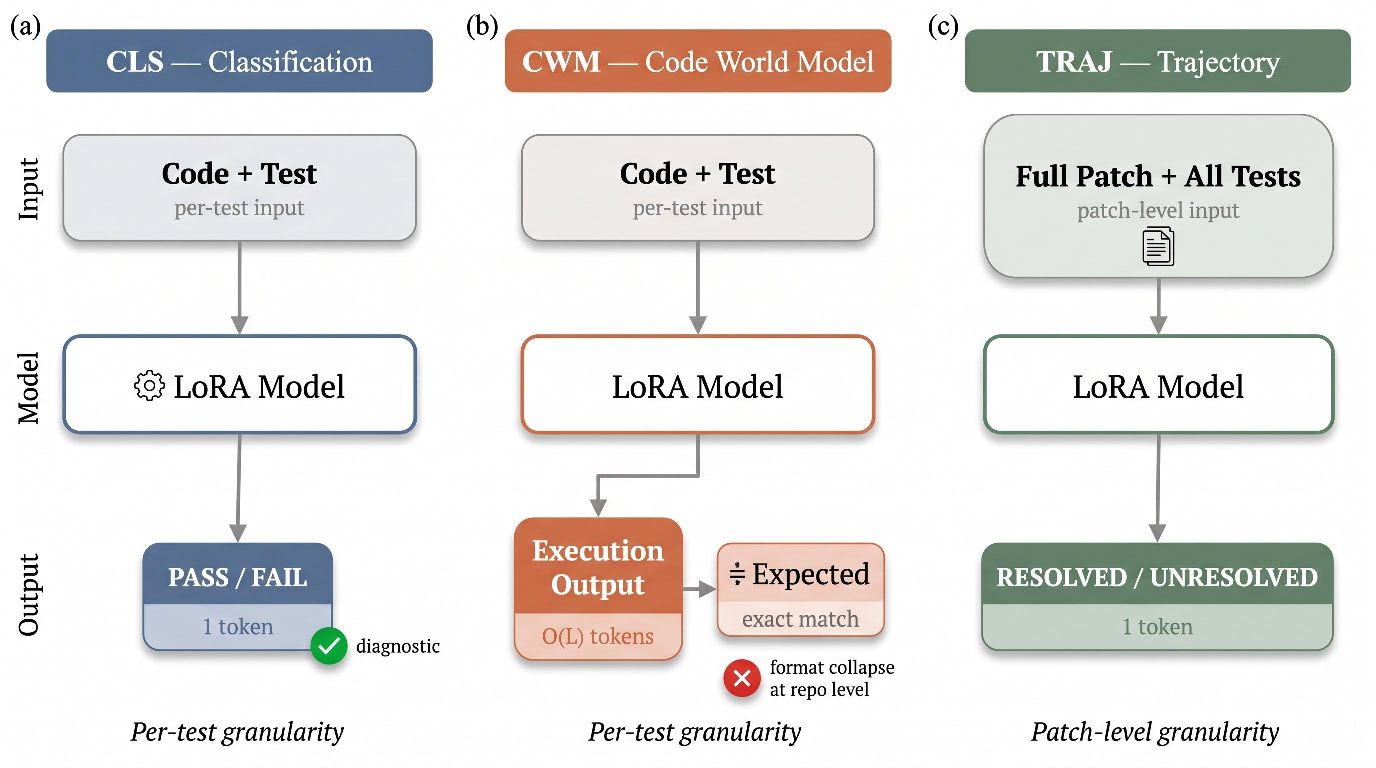
\includegraphics[width=\textwidth]{figures/paper/fig1_reformulation.pdf}
\caption{Three verification formulations. \textbf{Left:} \cls{} predicts binary pass/fail per test (1 output token). \textbf{Center:} \cwm{} generates execution output, derives verdict by exact match ($O(L)$ tokens). \textbf{Right:} Trajectory-level scoring predicts patch-level resolved/unresolved (1 token, no per-test signal). Each formulation makes different tradeoffs between output complexity, diagnostic granularity, and inference cost.}
\label{fig:reformulation}
\end{figure*}

\section{Method}
\label{sec:method}

Let $p$ denote a candidate patch and $T = \{t_1, \ldots, t_n\}$ its test suite, where each $t_i$ has label $y_i \in \{\text{\textsc{Pass}}, \text{\textsc{Fail}}\}$ from execution. Tests decompose into \emph{fail-to-pass} ($T_{\text{f2p}}$) and \emph{pass-to-pass} ($T_{\text{p2p}}$) subsets; a patch is correct iff $\forall\, t_i{:}\ y_i = \text{\textsc{Pass}}$. We compare three formulations for predicting correctness without execution.

\subsection{Verification Formulations}
\label{sec:formulations}

Let $c_p$ denote the code context (unified diff) of patch $p$.

\paragraph{\cls{} (per-test classification).} $f(c_p, t_i) \rightarrow \hat{y}_i \in \{\text{\textsc{Pass}}, \text{\textsc{Fail}}\}$ predicts a single binary token per test (cross-entropy loss). Patch verdict: $\hat{y}_p = \bigwedge_{i} [\hat{y}_i = \text{\textsc{Pass}}]$. Output cost: one token per test.

\paragraph{\cwm{} (output generation).}\footnote{We use ``code world model'' following \citet{meta2025cwm} to denote execution output prediction, distinct from world models in model-based reinforcement learning.} $g(c_p, t_i) \rightarrow \hat{o}_i \in \Sigma^*$ generates the execution output string (language modeling loss). Verdict by exact match: $\hat{y}_i = \text{\textsc{Pass}}$ iff $\hat{o}_i = o_i^*$.\footnote{Exact string matching is conservative, consistent with \citet{meta2025cwm}. Semantic equivalences are not counted.} When the generated output is unparseable (i.e., does not conform to the expected structured format), the prediction defaults to the majority class verdict. Output cost: $\sum_i |\hat{o}_i|$ tokens.

\paragraph{\traj{} (trajectory-level).} $h(c_p, T) \rightarrow \hat{y}_p \in \{\text{\textsc{Resolved}}, \text{\textsc{Unresolved}}\}$ predicts a single patch verdict from all tests and provides no per-test signal. \traj{} serves as a granularity control: \cls{}--\traj{} differences isolate the value of per-test decomposition independent of the classification formulation itself.

\subsection{Expected Failure Modes}
\label{sec:failure-modes}

Each formulation has characteristic failure modes that differ in their sensitivity to code complexity:

\paragraph{Generation failure modes (\cwm{}).} The open-ended output space introduces three failure modes: (1)~\emph{token-budget exhaustion}, where $|o_i^*| > B$ (generation budget in tokens) guarantees exact-match failure; (2)~\emph{string-value prediction errors}, where semantically equivalent outputs differing in surface form produce false negatives; and (3)~\emph{format compliance collapse}, where the model fails to produce structured predictions at high complexity. A token sequence of length $L$ with per-token accuracy $q$ has correct-sequence probability $q^L$, so long outputs are exponentially harder to predict exactly. We adopt exact string matching following \citet{meta2025cwm}; unparseable predictions default to the majority-class label (\textsc{Pass}).

\paragraph{Classification failure modes (\cls{}).} The single-token output eliminates format and truncation failures but constrains reasoning to internal representations. \cls{} errors manifest as false positives or false negatives; at function level, a mild FP bias (56.5\%) emerges.

\paragraph{Trajectory-level failure modes (\traj{}).} By collapsing per-test information into a single verdict, \traj{} discards diagnostic granularity but avoids per-test aggregation errors.

\paragraph{Complexity dependence.} When outputs are short (function level), generation modes (1)--(2) are rarely triggered and all formulations should perform comparably. As output complexity increases (repository level), generation-specific failures may compound. Whether this divergence is formulation-inherent or capacity-contingent is an empirical question (\S\ref{sec:experiments}).

\subsection{Oracle Accuracy-Utility Framework}
\label{sec:oracle}

For a buggy patch with $k = |T_{\text{f2p}}|$ fail-to-pass tests, a per-test verifier with recall $r$ detects the bug if it identifies at least one failing test: $P_{\text{detect}}(k) = 1 - (1 - r)^{k_{\text{eff}}}$, where $k_{\text{eff}} = k / (1 + (k-1)\rho)$ accounts for within-patch correlation via intraclass correlation coefficient (ICC) $\rho$~\citep{shrout1979icc}. The per-test advantage over a trajectory-level baseline ($a_h$) is $\Delta(k) = P_{\text{detect}}(k) - a_h$, with population expectation $\mathbb{E}[\Delta] = \sum_{k} P(|T_{\text{f2p}}| = k) \cdot \Delta(k)$. This predicts that per-test advantage concentrates in multi-F2P-test instances and vanishes at $k{=}1$, validated in \S\ref{sec:experiments} and Appendix~\ref{app:oracle}.


\section{Experiments}
\label{sec:experiments}

We systematically compare \cls{}, \cwm{}, and \traj{} across two representative code LLM families, two complexity levels, and multiple seeds to characterize the formulation landscape for neural code verification.

\subsection{Experimental Setup}
\label{sec:setup}

\paragraph{Datasets.}
\emph{Function-level}: mutated variants from HumanEval~\cite{chen2021humaneval} and MBPP~\cite{austin2021mbpp} (five mutation types), labels verified by execution. 19,076 samples (train 15,290 / val 1,896 / test 1,890; pass:fail $\approx$ 52:48, majority baseline 51.75\%).
\emph{Repo-level}: per-test instances from SWE-bench Verified~\cite{chowdhury2024swebenchverified} mutants. ${\sim}$70K training samples; val ($n{=}9{,}335$) and test ($n{=}9{,}784$) have zero problem overlap (majority baseline 72.96\%). Val-based checkpoint selection follows standard practice~\cite{jimenez2024swebench}; runs with NaN validation loss (due to truncated targets exceeding 2,048-token limits) default to the final epoch checkpoint (Appendix~\ref{app:hyperparams}). Qwen3 \cwm{} runs show early overfitting (best at ${\sim}$6\% of training); checkpoint details in Appendix~\ref{app:hyperparams}.

\paragraph{Models and training.}
We fine-tune Qwen3-4B and Qwen3-8B~\cite{qwen2025qwen3} with LoRA~\cite{hu2022lora} (rank 16, 3 epochs) across five seeds (3 bfloat16, 2 NF4 4-bit~\cite{dettmers2024qlora}). DeepSeek-Coder-6.7B~\cite{guo2024deepseekcoder} serves as a cross-model check (2 seeds). Our \cwm{} baseline uses LoRA fine-tuning for matched comparison, not the 32B CWM~\cite{meta2025cwm}. Zero-shot baselines use Qwen3-8B and Qwen3-32B (NF4). Full hyperparameters in Appendix~\ref{app:hyperparams}; prompts in Appendix~\ref{app:prompts}.

\paragraph{Statistics.}
Equivalence uses Two One-Sided Tests (TOST)~\cite{schuirmann1987tost} with $\pm$2\pp{} margin; seed-level paired analysis (df${=}$4 for 5-seed, df${=}$2 for 3-seed) treats each training seed as the unit of replication. Holm-Bonferroni correction~\cite{holm1979} controls family-wise error across the five primary comparisons (Table~\ref{tab:holm}). Confidence intervals use clustered bootstrap~\cite{davison1997bootstrap} (114 problem clusters, 10K resamples); intraclass correlation coefficient (ICC)~\cite{shrout1979icc} quantifies within-problem correlation. Bayesian Region of Practical Equivalence (ROPE) and mixed-effects regression supplement these tests. Full statistical power analysis in Appendix~\ref{app:power}.


\subsection{Function-Level Results}
\label{sec:func_results}

Table~\ref{tab:main_results} reports function-level results across formulations and model families.

\begin{table}[t]
\centering
\small
\caption{Function-level per-test accuracy on HumanEval+MBPP ($n{=}1{,}890$). Mean $\pm$ std over 5 seeds (Qwen3) or 2 seeds (DeepSeek). Seeds 42/123/456: bfloat16; 789/0: NF4. DeepSeek: $n{=}2$ seeds; std reported for descriptive comparison, not inferential. \traj{}\textsuperscript{$\star$} evaluated on 1,032-sample subset (447 matched variants). All prompting baselines use NF4 4-bit quantization. \textsuperscript{$\star$}Training configuration differs (\S\ref{sec:repo}).}
\label{tab:main_results}
\setlength{\tabcolsep}{6pt}
\renewcommand{\arraystretch}{1.0}
\begin{tabular}{llcc}
\toprule
\textbf{Method} & \textbf{Model} & \textbf{Seeds} & \textbf{Accuracy (\%)} \\
\midrule
\multicolumn{4}{l}{\emph{Qwen3 (primary)}} \\
\cls{} (fine-tuned) & 4B & 5 & \textbf{88.43 $\pm$ 0.78} \\
\cwm{} (fine-tuned) & 4B & 5 & \underline{87.19 $\pm$ 0.37} \\
\traj{}\textsuperscript{$\star$} (fine-tuned) & 4B & 5 & 86.30 $\pm$ 0.97 \\
\midrule
\multicolumn{4}{l}{\emph{DeepSeek-Coder (cross-model consistency check)}} \\
\cls{} (fine-tuned) & 6.7B & 2 & \textbf{86.85 $\pm$ 0.11} \\
\cwm{} (fine-tuned) & 6.7B & 2 & \underline{86.83 $\pm$ 1.49} \\
\traj{}\textsuperscript{$\star$} (fine-tuned) & 6.7B & 2 & 84.16 $\pm$ 1.30 \\
\midrule
\multicolumn{4}{l}{\emph{Prompting baselines}} \\
0-shot & 8B (Qwen3) & 1 & 60.53 \\
0-shot & 14B (Qwen3) & 1 & 66.24 \\
0-shot & 6.7B (DeepSeek) & 1 & 63.02 \\
Zero-shot LLM-as-judge & 8B (Qwen3) & 1 & 64.40 \\
Zero-shot LLM-as-judge & 6.7B (DeepSeek) & 1 & 56.56 \\
Zero-shot LLM-as-judge & 32B (NF4) & 1 & 71.69 \\
3-shot in-context learning & 8B (Qwen3) & 1 & 60.42 \\
3-shot in-context learning & 14B (Qwen3) & 1 & 73.12 \\
3-shot in-context learning & 6.7B (DeepSeek) & 1 & 59.95 \\
\midrule
Majority (pass) & --- & --- & 51.75 \\
\bottomrule
\end{tabular}
\end{table}

All three formulations achieve comparable accuracy on Qwen3-4B: \cls{} 88.43\%, \cwm{} 87.19\%, \traj{} 86.30\% (Table~\ref{tab:main_results}). The \cls{}--\cwm{} gap (0.02--1.24\pp{}) is within seed noise across both families; the \cls{}--\traj{} gap (2.13--2.69\pp{}) exceeds the $\pm$2\pp{} equivalence margin on DeepSeek-Coder (\S\ref{sec:equivalence}). Zero-shot baselines confirm that repo-level verification requires fine-tuning (35--36\pp{} gains) and that formulation choice matters only at repo level (\cls{} outperforms \cwm{} by 18--26\pp{}).


\subsection{Scaling Behavior}
\label{sec:scaling}

Beyond overall accuracy, we examine whether formulation ranking is stable across model sizes. Table~\ref{tab:scaling} compares all three formulations at 4B, 8B, and 14B. The 4B and 8B rows use seeds 42 and 123; the 14B row uses seeds 42, 123, and 456. All rows use bfloat16 inference.

\begin{figure}[t]
\centering
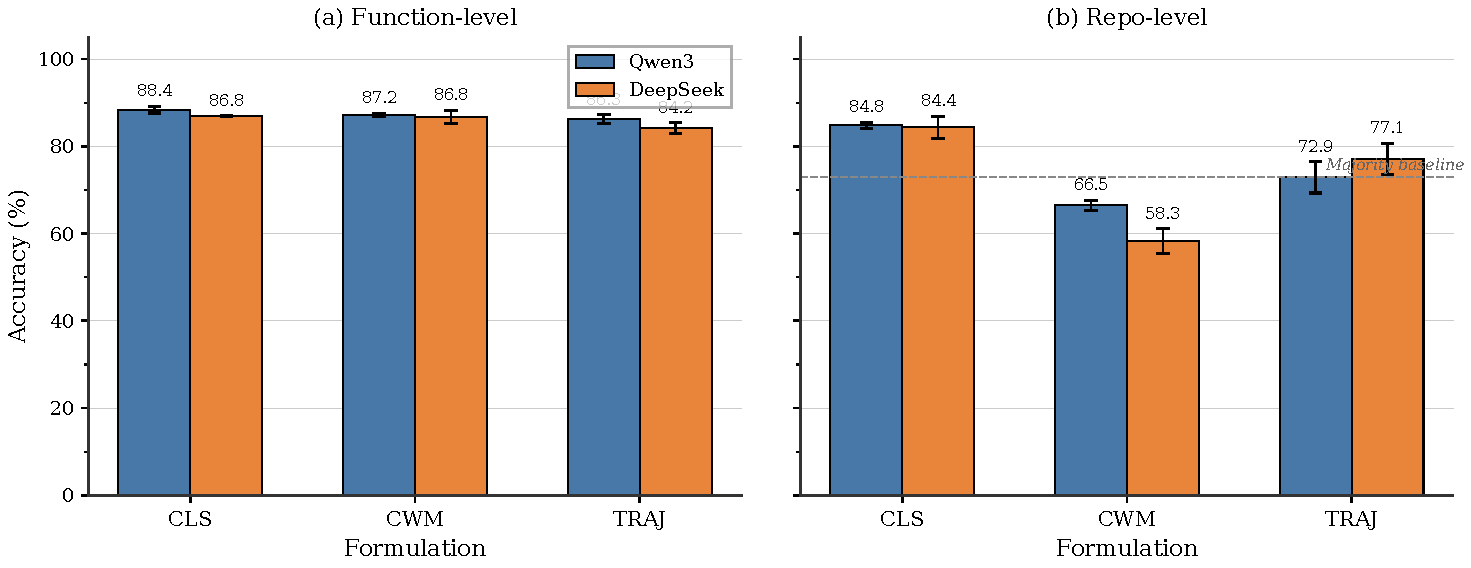
\includegraphics[width=0.82\columnwidth]{figures/paper/figure2_v3.pdf}
\caption{Function-level accuracy scaling (4B--14B). CLS and CWM accuracy with shaded gap region; $y$-axis does not start at zero. The \cls{}--\cwm{} gap shows a non-monotonic pattern: 1.32\pp{} at 4B, widening to 2.62\pp{} at 8B, then narrowing to 0.43\pp{} at 14B (3 seeds).}
\label{fig:scaling_gap}
\end{figure}

\cls{} and \traj{} both scale positively from 4B to 8B (+1.27\pp{} and +2.13\pp{} respectively), while \cwm{} remains flat ($-$0.03\pp{}). At 8B, the ranking is \cls{} (89.94) $>$ \traj{} (87.70) $>$ \cwm{} (87.33). The \cls{}--\cwm{} gap widens from 1.32\pp{} at 4B to 2.62\pp{} at 8B (Figure~\ref{fig:scaling_gap}); clustered bootstrap on the 3-seed superset (42, 123, 456 for \cls{}/\cwm{}) yields $p = 0.0066$ (95\% CI $[1.80, 2.71]$), which confirms the widening is not a sampling artifact.

At 14B (3 seeds), all three formulations converge in point estimates: \cls{} 89.93$\pm$0.80\%, \cwm{} 89.50$\pm$0.67\%, \traj{} 88.86$\pm$0.77\%. The maximum pairwise gap (\cls{}--\traj{}) narrows from 3.11\pp{} at 4B to 1.07\pp{} at 14B, within the $\pm$2\pp{} margin. Seed-level TOST (df${=}$2) is inconclusive in both pairs ($p{=}0.076$ for \cls{}--\cwm{}, $p{=}0.187$ for \cls{}--\traj{}), reflecting the low power of 3-seed comparisons; Bayesian ROPE provides moderate support ($P(\text{ROPE}){=}0.887$ and $0.780$; Appendix~\ref{app:bayesian_rope}). \cwm{}'s delayed scaling onset (flat 4B--8B, then +2.17\pp{} at 14B) and \traj{}'s decelerating convergence (+2.13\pp{} at 8B, +1.16\pp{} at 14B) are both consistent with capacity-dependent convergence at function level.

\paragraph{Baseline scaling.} Prompting baselines remain well below fine-tuning: the best result (14B 3-shot, 73.12\%) is 16.82\pp{} below fine-tuned \cls{} at 8B. Only \cls{} scales positively across both complexity levels; \traj{} shows negligible repo-level scaling (72.92\% at 4B, 73.61\% at 8B).


\subsection{Function-Level Equivalence}
\label{sec:equivalence}

We test pairwise equivalence on 523 variant-level instances across five seeds.\footnote{Seeds 789/0 use NF4 inference; the remaining three use bfloat16. Restricting to bfloat16 only: \cls{}--\cwm{} remains significant ($p{<}0.05$); \cls{}--\traj{} yields $p{=}0.128$.} Our Smallest Effect Size of Interest (SESOI) threshold of $\pm$2\pp{}~\cite{lakens2017,wellek2010} is domain-motivated but not pre-registered: at 85--88\% accuracy, 2\pp{} corresponds to ${\sim}$2--3 problems out of 114, below practitioner-relevant differences and consistent with between-seed variation (0.37--0.97\pp{} std). Within-problem predictions are correlated (ICC $= 0.191$, design effect [DEFF] $= 3.97$~\cite{moulton1990}); confidence intervals use clustered bootstrap (\S\ref{sec:setup}). Sensitivity analysis shows \cls{}--\cwm{} equivalence is robust across margins down to $\pm$1.63\pp{} (Table~\ref{tab:tost_sensitivity}, Figure~\ref{fig:tost_sensitivity}); \cls{}--\traj{} equivalence is margin-sensitive ($\pm$1.5\pp{}: $p{=}0.068$).

\paragraph{\cls{}--\cwm{} equivalence.} The pooled gap is 1.24\pp{} (88.43\%--87.19\%); TOST confirms equivalence at $p = 0.007$ ($\pm$2\pp{} margin), surviving Holm-Bonferroni correction ($k{=}5$, adjusted $p{=}0.028$; Table~\ref{tab:holm}). Equivalence holds at margins as tight as $\pm$1.63\pp{} (Appendix~\ref{app:tost_sensitivity}). On DeepSeek-Coder, the \cls{}--\cwm{} gap of 0.02\pp{} is consistent with equivalence but underpowered (2 seeds).

\paragraph{\cls{}--\traj{} equivalence.} The pooled gap is $-$0.45\pp{} (95\% CI [$-$1.71, +0.84]); TOST yields $p = 0.025$ ($\pm$2\pp{}), nominally significant but not surviving Holm-Bonferroni correction ($k{=}5$, adjusted $p{=}0.075$; Table~\ref{tab:holm}). The DeepSeek \cls{}--\traj{} gap (2.69\pp{}) exceeds the $\pm$2\pp{} margin; \traj{} parity is model-dependent. This holds under different training recipes (data volume and label granularity; \S\ref{sec:repo}). Per-test classification provides diagnostic information at no accuracy cost, paralleling process supervision~\cite{lightman2023letsverify}.

\begin{table}[t]
\centering
\small
\caption{Model-size scaling: accuracy (\%) at 4B, 8B, and 14B (Qwen3). Seeds 42/123 (4B/8B), seeds 42/123/456 (14B). All bfloat16 inference. $\Delta$: change from previous size. \cwm{} and \traj{}\textsuperscript{$\star$} use $n{=}2$ seeds (4B/8B) and $n{=}3$ seeds (14B). \traj{}\textsuperscript{$\star$} evaluated on 1{,}032-sample subset; \cls{}/\cwm{} use the full 1{,}890-sample set. \textsuperscript{$\star$}Training configuration differs (\S\ref{sec:repo}).}
\label{tab:scaling}
\setlength{\tabcolsep}{3pt}
\renewcommand{\arraystretch}{0.92}
\begin{tabular}{llccccc}
\toprule
\textbf{Method} & \textbf{Size} & \textbf{s42} & \textbf{s123} & \textbf{s456} & \textbf{Mean} & \textbf{$\Delta$} \\
\midrule
\multirow{3}{*}{\cls{}} & 4B & 87.83 & 89.52 & --- & \textbf{88.68} & --- \\
 & 8B & \textbf{90.48} & 89.40 & --- & \textbf{89.94} & +1.27 \\
 & 14B & 89.21 & \textbf{90.79} & 89.79 & \textbf{89.93 $\pm$ 0.80} & $-$0.01 \\
\midrule
\multirow{3}{*}{\cwm{}} & 4B & 87.51 & 87.20 & --- & \underline{87.36} & --- \\
 & 8B & 87.67 & 86.98 & --- & 87.33 & $-$0.03 \\
 & 14B & 89.26 & 88.99 & 90.26 & \underline{89.50 $\pm$ 0.67} & +2.17 \\
\midrule
\multirow{3}{*}{\traj{}} & 4B & 85.66 & 85.47 & --- & 85.57 & --- \\
 & 8B & 87.60 & 87.79 & --- & \underline{87.70} & +2.13 \\
 & 14B & 89.73 & 88.57 & 88.28 & 88.86 $\pm$ 0.77 & +1.16 \\
\bottomrule
\end{tabular}
\end{table}

\paragraph{Statistical power.} With $n_{\text{eff}} \approx 86$ after clustering, TOST power is ${\sim}$0.3~\cite{cohen1988}. The \cls{}--\cwm{} equivalence ($p{=}0.007$) is robust; the \cls{}--\traj{} inconclusive result (adjusted $p{=}0.075$) may reflect insufficient power ($n_{\text{eff}} \approx 350$ needed for ${\geq}$0.8 power). Bayesian ROPE corroborates: $P(\text{ROPE}){=}0.975$ for \cls{}--\cwm{}; \cls{}--\traj{} $P(\text{ROPE}){=}0.970$ at variant level but 0.542 at per-test level (Appendix~\ref{app:bayesian_rope}).


\subsection{Repo-Level: Complexity-Dependent Divergence}
\label{sec:repo}

Table~\ref{tab:repo_level} compares formulations at repository-level complexity. These results are established under ${\leq}$8B LoRA; preliminary 14B evidence (\S\ref{sec:scaling}) suggests these gaps may narrow at larger scales. Variant-level comparisons ($n{=}48$) are exploratory due to limited seed coverage; the per-test interaction effect is statistically confirmed (below). Checkpoints are val-selected where validation loss is computable (\S\ref{sec:setup}); the test set has zero problem overlap with validation.

\begin{table}[t]
\centering
\small
\caption{Repo-level cross-formulation comparison on SWE-bench Verified test set. Qwen3-8B \cls{}/\traj{}: mean $\pm$ std over 3 seeds; DeepSeek \cls{}: 2 seeds\textsuperscript{$\ddagger$}; DeepSeek \traj{}: 3 seeds; Qwen3-4B: seed 42. \cwm{}: 3 seeds (42/123/456).}
\label{tab:repo_level}
\setlength{\tabcolsep}{5pt}
\renewcommand{\arraystretch}{1.0}
\begin{tabular}{lcccc}
\toprule
\textbf{Model} & \textbf{\cls{} (\%)} & \textbf{\cls{} Var.\ (\%)} & \textbf{\cwm{} (\%)} & \textbf{\traj{} Var.\ (\%)\textsuperscript{$\diamond$}} \\
\midrule
Qwen3-4B & 83.63 & 64.58 & 58.04 & 72.92 \\
Qwen3-8B & \textbf{84.83 $\pm$ 0.67} & 72.92 / 81.25\textsuperscript{$\dagger$} & 66.48 $\pm$ 1.14 & 73.61 $\pm$ 3.18 \\
DeepSeek-6.7B & 84.38 $\pm$ 2.50\textsuperscript{$\ddagger$} & 81.25\textsuperscript{$\dagger$} & 58.30 $\pm$ 2.82 & 77.08 $\pm$ 3.61 \\
\midrule
0-shot (Qwen3-8B) & 49.90 & --- & --- & --- \\
0-shot (DeepSeek) & 48.54 & --- & --- & --- \\
Majority & 72.96 & 54.17 & 72.96 & 54.17 \\
\bottomrule
\end{tabular}

\vspace{2pt}
{\footnotesize
\textsuperscript{$\dagger$}Individual-seed variant accuracy.\\
\textsuperscript{$\ddagger$}One seed excluded: target truncation (sequences exceeding 2,048 tokens)$\to$NaN val loss, decision collapse (near-zero fail recall; Table~\ref{tab:taxonomy}); mean over two matched seeds.\\
\textsuperscript{$\diamond$}Var.\ columns: variant-level accuracy ($n{=}48$); \cls{} aggregated via all-pass rule; \traj{} by design. Per-test: $n{=}9{,}784$. \cwm{} unparseable: 54\% (4B); default to pass; parseable-only 38--43\%, below majority. Eval seq\_length differs across models (Appendix~\ref{app:threats}). \cwm{} uses final-epoch checkpoint (step 6633) for s123/s456; s42 uses an earlier checkpoint (step 400) from a prior training configuration. Val loss is undefined for DeepSeek \cwm{} runs (Qwen3 \cwm{} has valid val loss; see \S\ref{sec:setup}). Checkpoint sensitivity analysis in Appendix~\ref{app:cwm_convergence}.}
\end{table}

Few-shot prompting (3-shot in-context learning) collapses to an always-predict-unresolved baseline (variant accuracy 45.83\%, below majority 54.17\%; Appendix~\ref{app:few_shot}); execution-free verification requires task-specific fine-tuning regardless of formulation, yielding 35--36\pp{} gains (Table~\ref{tab:repo_level}) before formulation choice becomes relevant.

\paragraph{Formulation divergence.} Under our 4--8B LoRA protocol, \cls{} and \cwm{} diverge: the gap is 25.59\pp{} at 4B and 18.35\pp{} at 8B (Table~\ref{tab:repo_level}), with \cwm{} falling below majority baseline at both scales. Limited seed coverage and multiple confounds (see \hyperref[sec:threats]{Threats to Validity} in the appendix) limit causal attribution.

\paragraph{Cross-model consistency.} DeepSeek-Coder shows the same direction (\cls{} $>$ \cwm{}) across all seeds; gap variation across families (20\pp{} Qwen3 vs.\ 23--28\pp{} DeepSeek) narrows to ${\sim}$2\pp{} under matched checkpoints (Appendix~\ref{app:threats}). All six \cwm{} repo-level seeds exhibit format collapse ($>$50\% unparseable), ruling out seed-specific artifacts.

\paragraph{Failure mode taxonomy.} Variant-level analysis ($n{=}48$) identifies three failure modes (Table~\ref{tab:taxonomy}; full variant-level and per-mutation breakdowns in Appendices~\ref{app:variant_level} and~\ref{app:repo_mutation}): format collapse (\cwm{}, 53--74\% unparseable), decision collapse (\cls{} under truncate preprocessing, fail recall ${\sim}$14\%), and aggregation penalty (\cls{} under drop preprocessing, fail recall 38--57\%). Decision collapse is configuration-dependent, not model-inherent. \traj{} avoids aggregation penalty by predicting variant outcomes directly (72.92--77.08\%); downsampling \cls{} to match \traj{}'s data volume still yields 80.74\% (+7.82\pp{} above \traj{}; Appendix~\ref{app:downsample}). The \cls{}--\traj{} repo-level comparison remains exploratory: the downsample ablation controls data volume but not label granularity (per-test vs.\ variant-level), a formulation-inherent confound.

\paragraph{Default assignment artifact.} The apparent \cwm{} accuracy increase from 4B to 8B is an artifact of rising unparseable rate (53.7\%$\to$73.8\%), inflating accuracy via majority-class default while parseable-only accuracy decreases (42.88\%$\to$38.52\%); cross-seed evidence confirms the pattern (Appendix~\ref{app:parseable_bias}).

\paragraph{Complexity as moderator.} The \cls{}--\cwm{} gap widens from 1--3\pp{} (function) to 18--26\pp{} (repo) under our protocol; a matched-context ablation confirms input disparity explains $<$3\% of this gap (Appendix~\ref{app:ablations}). While the directional advantage of lower-complexity output formulations is anticipated from \S\ref{sec:failure-modes}, the magnitude of this gap, the function-level equivalence, and the specific failure mechanisms (Table~\ref{tab:taxonomy}) were not predictable a priori.

\paragraph{Formulation$\times$complexity interaction.} A mixed-effects linear probability model (LPM) ($n{=}56{,}480$, 139 clusters, DeepSeek-Coder) confirms: \cwm{} effect at function level is negligible ($\hat{\beta}{=}-0.002$, $p{=}0.805$), but the formulation$\times$complexity interaction is highly significant ($z{=}-23.7$, $p{<}0.001$). A cross-model LPM confirms formulation dominates ($\hat{\beta}{=}-0.22$ vs.\ model $\hat{\beta}{=}+0.011$); model identity significance is estimator-dependent (LPM $p{=}0.002$; generalized estimating equations [GEE] $p{=}0.449$), consistent with limited clusters ($k{=}25 < 40$; Appendix~\ref{app:interaction}).

\begin{table}[t]
\centering
\small
\caption{Repo-level failure mode taxonomy. Variant-level majority baseline: 54.17\%.}
\label{tab:taxonomy}
\setlength{\tabcolsep}{6pt}
\renewcommand{\arraystretch}{1.0}
\begin{tabular}{llcc}
\toprule
\textbf{Failure Mode} & \textbf{Representative} & \textbf{Fail Recall} & \textbf{Variant Acc} \\
\midrule
Format collapse & \cwm{} (all) & N/A & 48--52\% \\
Decision collapse & \cls{} (DeepSeek, s123) & ${\sim}$14\% & 56\% \\
Aggr.\ penalty & \cls{} (Qwen3-8B) & 51--57\% & 73--81\% \\
Aggr.\ penalty & \cls{} (DeepSeek, s42) & 38--51\% & 79--81\% \\
\bottomrule
\end{tabular}
\end{table}



\section{Conclusion}
\label{sec:conclusion}

We presented the first systematic comparison of three execution-free verification formulations (\cls{}, \cwm{}, \traj{}) under ${\leq}$8B LoRA fine-tuning. At function level, \cls{} and \cwm{} are statistically equivalent (TOST $p{=}0.007$, 5 seeds); \traj{} equivalence is inconclusive after Holm correction. At repository level, divergence reaches 18--26\pp{} via three failure modes; the formulation$\times$complexity interaction is highly significant ($z{=}-23.7$, $p{<}0.001$), consistent across families. 14B results narrow function-level gaps to ${\sim}$1\pp{}; whether repo-level divergence is formulation-inherent or capacity-contingent remains open. Scaling to 32B+~\cite{meta2025cwm} and complexity-aware routing are key open questions.

\section*{Limitations}

Primary findings use ${\leq}$8B LoRA fine-tuning with multi-seed replication; 14B results use a single model family with 3 seeds; cross-family replication at 32B+ is needed. The repo-level gap may diminish with scale or execution-trace pretraining~\cite{meta2025cwm}. All evaluation uses Python-only benchmarks; training data uses synthetic mutation operators~\cite{andrews2005mutation,just2014mutants} with untested transfer to real faults (Appendix~\ref{app:limitations}). Constrained decoding~\cite{poesia2022synchromesh,dong2024xgrammar,willard2023outlines} may mitigate \cwm{}'s format collapse but was not evaluated.


\bibliographystyle{icais_conference}
\bibliography{references}

\appendix
\renewcommand{\thesection}{\AlphAlph{\value{section}}}
% ICAIS 2026 Track 1 statements. Copy this file into each standalone
% submission package and include it before the bibliography.
\section*{ICAIS Track 1 Statements}

\paragraph{AI System Disclosure.}
For this revision, OpenAI Codex was used to inspect the LaTeX sources,
diagnose compilation and formatting issues, and assist with manuscript-level
language and typesetting edits. It did not originate the reported
measurements or independently validate the empirical claims. AI systems used
as experimental subjects or research tools are identified in the paper where
they affect the methods or interpretation. No AI system is listed as an
author.

\paragraph{Human Accountability Statement.}
The human authors retain sole responsibility for the research questions,
methodology, data, analyses, claims, citations, ethical compliance, and final
submission. They are responsible for checking all AI-assisted edits and for
correcting any remaining errors.

\paragraph{Evidence of Scientific Validity.}
The main paper reports the study design, evaluation protocol, quantitative
evidence, and limitations supporting its claims. The appendix provides
additional experimental details, robustness or sensitivity analyses, and
reproducibility information where applicable. Claims should be interpreted
within the scope and limitations stated in the paper.

\section*{Analysis}
\phantomsection\label{sec:analysis}

\paragraph{Aggregation penalty.} The aggregation penalty ranges from 1.36\pp{} to 19\pp{}, negligible at function level ($\bar{T} \approx 2.3$) but substantial at repo level ($\bar{T} \gg 10$; Appendix~\ref{app:extended_analysis}(a)).

\begin{figure}[t]
\centering
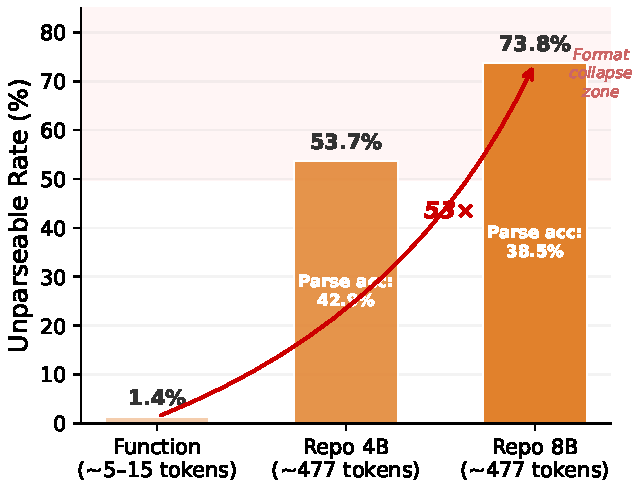
\includegraphics[width=0.72\columnwidth]{figures/paper/fig_cwm_unparseable.pdf}
\caption{\cwm{} unparseable rate by complexity level. Function-level outputs (${\sim}$5--15 tokens) yield 1.4\% unparseable; repo-level outputs (${\sim}$477 tokens) reach 53.7\% (4B) and 73.8\% (8B). Parseable-only accuracy (inside bars) decreases from 4B to 8B despite rising overall accuracy---evidence of default-assignment inflation.}
\label{fig:cwm_unparseable}
\end{figure}

\paragraph{Why does generation degrade at repo level?} Output complexity increases nonlinearly: function-level outputs average ${\sim}$5--15 tokens; repo-level outputs average ${\sim}$477 tokens (Figure~\ref{fig:cwm_unparseable}), leading to format collapse (53--74\% unparseable; Appendix~\ref{app:qualitative}). Even parseable outputs achieve only 38--43\%, below majority; a model accidentally trained on CLS-format data achieves 86.05\% with 0\% unparseable; this confirms that degradation stems from output format complexity, not task difficulty (Appendix~\ref{app:extended_analysis}(c)). Four targeted interventions all fail to close this gap (Appendix~\ref{app:extended_analysis}(g)). \cls{} achieves 217$\times$ higher throughput (1 vs.\ avg 477 output tokens).

\begin{figure}[t]
\centering
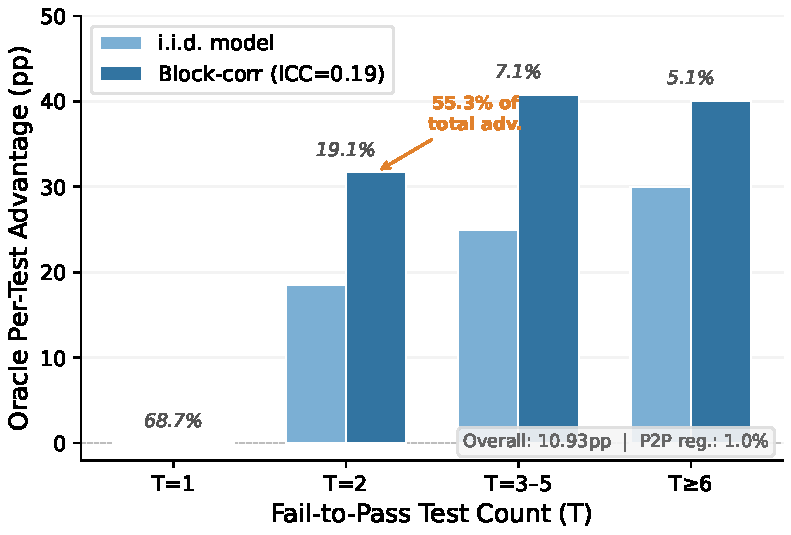
\includegraphics[width=0.82\columnwidth]{figures/paper/fig3_oracle_stratified.pdf}
\caption{Oracle per-test advantage by F2P test count $T$. Advantage is zero at $T{=}1$ (68.7\% of instances) and concentrates at $T{=}2$ (19.1\%, contributing 55.3\% of total advantage).}
\label{fig:oracle_stratified}
\end{figure}

\paragraph{Error complementarity.} \cls{} and \cwm{} make partially complementary errors. An oracle combination achieves 90.63\% (+2.80\pp{}; 95\% CI [89.3\%, 91.9\%]; single-seed) at function level and 95.83\% (+14.58\pp{}; $n{=}48$) at repo level (Figure~\ref{fig:oracle_stratified}). Simple routing heuristics capture $<$0.4\pp{} of the oracle gap; the complementarity is instance-specific, so simple heuristics are insufficient. Whether a learned router can capture this advantage remains open (Appendix~\ref{app:oracle}).

\section*{Threats to Validity}
\phantomsection\label{sec:threats}

We identify five potential confounds (Appendix~\ref{app:threats}): checkpoint selection ($<$1\pp{}), evaluation sequence length (${\sim}$1.5\pp{}), preprocessing (${\sim}$8\pp{}; val-test distribution shift in Appendix~\ref{app:mutation_distribution}), \traj{} training regime, and \cwm{} scale/pretraining (primary limitation). Preprocessing and checkpoint interact, accounting for up to 7.68\pp{} variation within one model (Appendix~\ref{app:threats}). The 18--26\pp{} gap exceeds any single confound, but correlated confounds and limited seeds preclude definitive causal attribution. Holm-Bonferroni ($k{=}5$) confirms the two core claims (adjusted $p{=}0.015$ and $p{=}0.028$; Table~\ref{tab:holm}).

\begin{table}[t]
\centering
\small
\caption{Holm-Bonferroni correction for primary comparisons ($k{=}5$). Comparisons ranked by raw $p$-value; each tested against $\alpha / (k - \text{rank} + 1)$.}
\label{tab:holm}
\setlength{\tabcolsep}{3pt}
\resizebox{\columnwidth}{!}{%
\begin{tabular}{clcccc}
\toprule
\textbf{Rank} & \textbf{Comparison} & \textbf{Raw $p$} & \textbf{Factor} & \textbf{Adj $p$} & \textbf{Sig.?} \\
\midrule
1 & Repo: \cls{} vs \cwm{} & 0.003 & $\times$5 & 0.015 & \checkmark \\
2 & Func: \cls{} vs \cwm{} (TOST $\pm$2\pp{}) & 0.007 & $\times$4 & 0.028 & \checkmark \\
3 & Func: \cls{} vs \traj{} (TOST $\pm$2\pp{}) & 0.025 & $\times$3 & 0.075 & --- \\
4 & Repo: \cwm{} vs \traj{} & 0.039 & $\times$2 & 0.078 & --- \\
5 & Repo: \cls{} vs \traj{} & 0.385 & $\times$1 & 0.385 & --- \\
\bottomrule
\end{tabular}}
\end{table}


\section*{Related Work}
\phantomsection\label{sec:related_work}

\paragraph{Execution Simulation and Verification.}
Execution trace generation improves code reasoning~\cite{nye2021scratchpad}, with extensions to output prediction~\cite{meta2025cwm,maimon2026selfexecution,liu2024codemind,liu2023codeexecutor,lee2026solidcoder}, failure analysis~\cite{abdollahi2025demystifying}, and error detection~\cite{li2024redo}. CRUXEval~\citep{gu2024cruxeval} benchmarks code execution prediction at function level; RepoExec~\citep{nam2025repoexec} evaluates repo-level code generation with execution-based correctness checks. Our work extends execution prediction to repo-level repair verification. Verification formulations span trajectory-level reward~\cite{shum2025swerm}, process-level feedback~\cite{li2025codeprm,xu2025patchreasoner}, per-test classification~\cite{ni2023lever,chen2023codet}, learned metrics~\cite{zhuo2024icescore,dong2024codescore,zhou2023codebertscore}, and RL with execution-based rewards~\cite{wang2026verpo,tang2026execverify}. Aletheia~\cite{venkatkrishna2026aletheia} compares training recipes; we compare \emph{formulations}. Test-time scaling~\cite{snell2024scaling,li2025sstar,chen2025vgsearch} and self-consistency~\cite{wang2023selfconsistency} demonstrate verification value; none compare formulations at matched capacity.

\paragraph{Process vs.\ Outcome Supervision.}
PRMs outperform ORMs for math reasoning~\cite{lightman2023letsverify,uesato2022solving}, with code-specific extensions~\cite{ye2025prlcoder,zhang2026funprm,jiang2025coderlplus,li2025codeprm}. GenRM~\cite{hosseini2025genrm} and GenPRM~\cite{zhao2026genprm} show generative verifiers outperform discriminative ones for math; our results reveal a domain difference---in code, the generative formulation does not outperform classification, which points to domain-specific tradeoffs (Appendix~\ref{app:threats}). In reward modeling terms, \cls{} maps to PRM, \traj{} to ORM, and \cwm{} to generative verification~\cite{hosseini2025genrm}; we also vary output format.

\paragraph{Repair, Mutation Testing, and Task Framing.}
CodeRL~\cite{le2022coderl}, AlphaCode~\cite{li2022alphacode,alphacode2023team}, and Reflexion~\cite{shinn2023reflexion} use execution feedback for repair. SWE-bench~\cite{jimenez2024swebench,chowdhury2024swebenchverified} benchmarks and SWE-agent~\cite{yang2024sweagent}/Agentless~\cite{xia2024agentless} demonstrate pipelines where verification is a bottleneck~\cite{yang2025aprsurvey}. Predictive mutation testing~\cite{tufano2019predictive,kim2022predictive,wang2024llmmutation,jain2023contextual} shares our per-test structure. \citet{raffel2020t5} showed that task framing affects NLP performance; we find that complexity moderates the classification--generation tradeoff in code verification.



% Responsible-research checklist (if required) is completed in the submission form, not in the PDF
% \input{checklist}

\appendix

\noindent\textbf{Appendix overview.} A: Oracle analysis. B: Ablations. C: Per-mutation breakdown. D: Variant-level accuracy. E: Hyperparameters. F: Prompt templates. G: Mutation distribution. H: Qualitative errors. I: Extended analysis (I.a--I.k). J: TOST sensitivity (J.1: Bayesian ROPE). K: Effect sizes. L: Holm-Bonferroni. M: Mixed-effects regression. N: Parseable bias. O: Threats (O.1: CWM convergence; O.2: Extended validity). P: AI assistants.

\section{Oracle Accuracy-Utility Analysis}
\label{app:oracle}

We stratify SWE-bench Verified instances by Fail-to-Pass (F2P) test count $T$, comparing per-test vs.\ trajectory-level oracle resolve rates under i.i.d.\ and block-correlated error models (ICC $= 0.191$, from function-level analysis; \S\ref{sec:equivalence}).

\begin{table}[h]
\centering
\small
\caption{Oracle accuracy-utility frontier: per-test advantage stratified by F2P test count ($T$) on SWE-bench Verified (500 instances). Block-correlated model uses function-level ICC $= 0.191$ (from function-level analysis, \S\ref{sec:equivalence}). Pass-to-Pass (P2P) regression rate: 1.04\% mean, 0\% median.}
\label{tab:oracle}
\setlength{\tabcolsep}{6pt}
\begin{tabular}{lcccc}
\toprule
\textbf{$T$} & \textbf{Inst.\%} & \textbf{i.i.d.\ (\pp{})} & \textbf{Block (\pp{})} & \textbf{Contrib.\%} \\
\midrule
$1$ & 68.7 & $-$0.04 & $-$0.09 & $\approx$0 \\
$2$ & 19.1 & 18.49 & 31.69 & 55.3 \\
$3$--$5$ & 7.1 & 25.00 & 40.74 & $\approx$26 \\
$\geq 6$ & 5.1 & 30.00 & 40.06 & $\approx$19 \\
\midrule
\textbf{All} & 100.0 & --- & \textbf{10.93} & 100.0 \\
\bottomrule
\end{tabular}
\end{table}

Figure~\ref{fig:oracle_stratified} (main text) shows the oracle per-test advantage by F2P test count.

Table~\ref{tab:oracle} and Figure~\ref{fig:oracle_stratified} reveal a sharp concentration: at $T = 1$ (68.7\% of instances), per-test and trajectory-level are informationally equivalent. The advantage materializes at $T = 2$ (19.1\%), where block-correlated advantage reaches 31.69\pp{} (55.3\% of total). The overall block-correlated advantage is 10.93\pp{}, driven by the $T \geq 2$ minority. Block correlation amplifies relative to i.i.d.: at $T = 2$, 31.69\pp{} vs.\ 18.49\pp{} (1.7$\times$). P2P regression is negligible (1.04\% mean, 0\% median); the practical value concentrates in F2P discrimination.

\paragraph{Sensitivity to ICC estimate.}
The analysis above uses ICC $= 0.191$ from function-level analysis (\S\ref{sec:equivalence}), where mean cluster size $\bar{k} \approx 16.5$ yields DEFF $= 3.97$. At repository level, within-problem correlation is substantially stronger: ICC $= 0.3146$ with DEFF $= 114.4$ (\S\ref{sec:repo}), yielding an effective sample size of $n_{\text{eff}} \approx 9{,}784 / 114.4 \approx 86$ independent observations~\cite{moulton1990}, still sufficient for regression but limiting precision of variance component estimates. This is a consequence of the larger and more heterogeneous test suites in SWE-bench Verified problems. Under higher ICC, within-problem errors cluster more tightly and amplify the block-correlated per-test advantage at each $T$ stratum; the correction from i.i.d.\ to block-correlated grows monotonically with ICC. The function-level ICC $= 0.191$ used in Table~\ref{tab:oracle} thus provides a conservative lower bound on the per-test advantage. The repo-level correlation structure would yield an even larger gap between per-test and trajectory-level oracle resolve rates, which strengthens the case for per-test granularity at repository-level complexity.

\section{Ablation Studies}
\label{app:ablations}

\paragraph{LoRA rank sensitivity.}
All \cwm{} experiments use LoRA rank $r{=}16$. To test whether this capacity constraint handicaps \cwm{}, we train rank-32 variants (seed 42), doubling adapter parameters.

\begin{table}[h]
\centering
\small
\caption{LoRA rank ablation for \cwm{} 4B (seed 42, 3 epochs, lr $= 2{\times}10^{-4}$). Rank-16 seed variance: 0.53\pp{} (seeds 42 vs.\ 456).}
\label{tab:rank_ablation}
\setlength{\tabcolsep}{4pt}
\begin{tabular}{lccccc}
\toprule
\textbf{Config} & \textbf{$\alpha/r$} & \textbf{Acc (\%)} & \textbf{Fail \fone{}} & \textbf{Pass \fone{}} & \textbf{$\Delta$} \\
\midrule
$r{=}16$, $\alpha{=}32$ & 2 & \textbf{87.51} & --- & --- & --- \\
$r{=}32$, $\alpha{=}32$ & 1 & 87.00 & 87.1 & 86.9 & $-$0.51 \\
$r{=}32$, $\alpha{=}64$ & 2 & 87.04 & 87.27 & 86.79 & $-$0.47 \\
\bottomrule
\end{tabular}
\end{table}

Both rank-32 variants fall within the 2-seed variance of the rank-16 baseline (0.53\pp{} between seeds 42 and 456; Table~\ref{tab:rank_ablation}). The $\alpha{=}64$ variant (matching the baseline $\alpha/r{=}2$ ratio) rules out the confound that the $\alpha{=}32$ result might reflect reduced effective scaling rather than rank insensitivity. This is consistent with \cwm{}'s function-level performance being bounded by output-format constraints rather than adapter capacity.

\paragraph{Majority voting.}
Majority voting ($K{=}3$) decreases accuracy from 87.51\% to 86.83\% ($-$0.68\pp{}): errors are systematic rather than stochastic, so sampling-based ensembles do not help.

\paragraph{Sequence-length ablation details.}
Both formulations are trained with \texttt{max\_seq\_length}$=$2,048. At inference, \cwm{} reserves \texttt{max\_new\_tokens}$=$512, leaving ${\sim}$1,536 effective input tokens; \cls{} allocates nearly all context to input (5,120--8,192 tokens). A matched-context ablation (\cls{} 8B at 2,048 tokens) achieves 83.04\%, only 1.44\pp{} below the 8,192-token evaluation (84.48\%), though truncation introduces 136 unparseable outputs (1.39\% of test samples). The matched-context gap (\cls{}@2,048 vs.\ \cwm{}@2,048) is 25.00\pp{} (98\% of the full 25.59\pp{} gap), confirming that input context disparity explains at most 3\% of the difference.

\paragraph{Training data size control.}
\label{app:downsample}
To control for the training set size asymmetry between \cls{} (${\sim}$70K instances) and \traj{} (386 variant-level instances, ${\sim}$8K per-test equivalents, at repo level), we downsample \cls{} training data to match \traj{} in data volume. Downsampled \cls{} (Qwen3-4B, seed 42) achieves 80.74\% repo-level per-test accuracy, only 2.89\pp{} below the full-data \cls{} (83.63\%) and still 7.82\pp{} above \traj{} (72.92\%). The \cls{} formulation advantage is not attributable to training data volume.

At function level, the relationship reverses: \traj{} uses 8,052 variant-level instances (2.24$\times$ more unique variants than \cls{}/\cwm{}'s 3,596 from 15,290 per-test instances). \cls{} nonetheless outperforms \traj{} by 2.13\pp{} (88.43\% vs.\ 86.30\%, Qwen3-4B), ruling out data volume as the explanation. An extreme downsample ablation (CLS trained on 447 per-test instances, ${\sim}$105 unique variants) achieves 78.57 $\pm$ 0.78\%, confirming that per-test classification maintains reasonable performance under severe data reduction, though it falls below \traj{} (86.30\%) given the 20$\times$ data disadvantage.

\paragraph{Few-shot prompting baselines.}
\label{app:few_shot}
We evaluate 3-shot in-context learning at repo level to test whether prompting strategy closes the gap to fine-tuned models. Table~\ref{tab:few_shot} reports both per-test and variant-level accuracy.

\begin{table}[h]
\centering
\small
\caption{Repo-level prompting baselines (per-test $n{=}9{,}784$; variant-level $n{=}48$). Majority baseline: 72.96\% per-test, 54.17\% variant-level.}
\label{tab:few_shot}
\setlength{\tabcolsep}{6pt}
\begin{tabular}{lccc}
\toprule
\textbf{Model} & \textbf{0-shot (per-test)} & \textbf{3-shot (per-test)} & \textbf{3-shot (variant)} \\
\midrule
Qwen3-8B & 49.90\% & 71.61\% & 45.83\%\textsuperscript{$\ast$} \\
DeepSeek-6.7B & 48.54\% & 46.28\% & 45.83\%\textsuperscript{$\ast$} \\
\bottomrule
\end{tabular}

\vspace{2pt}
{\footnotesize \textsuperscript{$\ast$}Both models achieve 45.83\% by correctly classifying all 22 unresolved variants and zero resolved variants (22/48 = 45.83\%), equivalent to an always-predict-unresolved baseline. The 100\% overlap in variant-level predictions confirms complete degradation at task-relevant granularity.}
\end{table}

Both models converge to exactly 45.83\% variant-level accuracy under 3-shot prompting, below majority baseline (54.17\%). Variant-level analysis reveals this is not a coincidence: both models correctly classify all 22 unresolved variants and zero resolved variants, equivalent to an always-predict-unresolved baseline with 100\% prediction overlap. Per-test accuracy diverges sharply (Qwen3-8B 71.61\% vs.\ DeepSeek 46.28\%), but this divergence is entirely superficial: Qwen3-8B predicts pass on nearly all tests, inflating per-test accuracy on a pass-heavy dataset (72.96\% pass rate) without genuine discriminative ability. Per-test metrics can thus severely misrepresent baseline capability; variant-level evaluation is necessary to detect complete degradation. Neither 0-shot nor few-shot prompting approaches fine-tuned performance (82--84\% per-test); fine-tuning is a necessary condition for repo-level verification.

\section{Repo-Level Per-Mutation Breakdown}
\label{app:repo_mutation}

Table~\ref{tab:mutation_breakdown} compares per-mutation accuracy at repo level. \cls{} produces 0\% unparseable outputs; all values are direct classification accuracy. \cwm{} overall accuracy includes default-pass assignment for unparseable outputs (see \S\ref{sec:repo}).

\begin{table}[h]
\centering
\small
\caption{Per-mutation test accuracy (\%) at repo level (SWE-bench Verified, $n{=}9{,}784$). \cls{} 8B reports two seeds; $\Delta$ is mean 4B$\to$8B gain for \cls{}. \cwm{} 4B per-mutation overall accuracy omitted for non-gold mutations due to low parse rates (4.4--56.9\%, Table~\ref{tab:cwm_mutation_parse}); gold overall accuracy derived from parse rate 43.5\% and parseable accuracy 23.5\%.}
\label{tab:mutation_breakdown}
\resizebox{\columnwidth}{!}{%
\setlength{\tabcolsep}{3pt}
\begin{tabular}{lccccccc}
\toprule
\textbf{Mutation} & \textbf{$n$} & \textbf{CLS 4B} & \textbf{CLS 8B s42} & \textbf{CLS 8B s123} & \textbf{CWM 4B} & \textbf{CWM 8B} & \textbf{$\Delta$ CLS} \\
\midrule
gold & 4,633 & 98.25 & 96.24 & 99.60 & 66.72 & 80.06 & $-$0.33 \\
operator\_swap & 3,357 & 78.91 & 81.38 & 82.60 & --- & 54.57 & +3.08 \\
off\_by\_one & 183 & 58.47 & 86.89 & 79.20 & --- & 63.39 & \textbf{+24.58} \\
return\_value & 562 & 67.97 & 75.44 & 66.40 & --- & 49.11 & +2.95 \\
boundary\_removal & 1,049 & 46.90 & 46.90 & 44.90 & --- & 42.23 & $-$1.00 \\
\bottomrule
\end{tabular}}
\end{table}

Figure~\ref{fig:mutation_heatmap} visualises the per-mutation accuracy contrast between \cls{} and \cwm{} at repo level.

\begin{figure}[h]
\centering
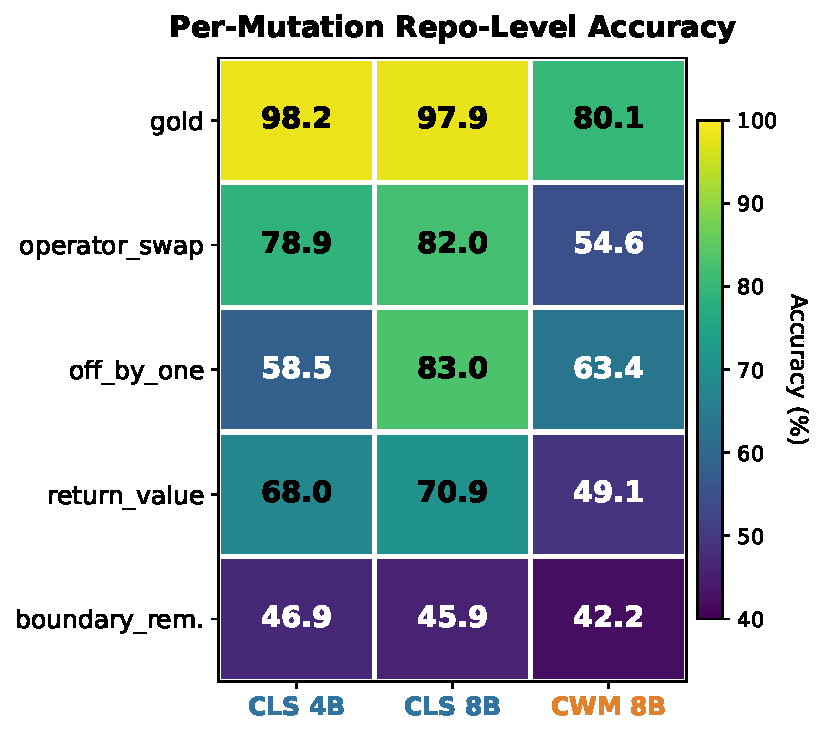
\includegraphics[width=0.7\columnwidth]{figures/paper/fig_mutation_heatmap.pdf}
\caption{Per-mutation repo-level accuracy heatmap. \cls{} 8B values are seed-averaged (s42/s123). \cwm{} 8B includes default-pass for unparseable outputs. \texttt{boundary\_removal} is a scale-invariant difficulty ceiling (${\sim}$45\%) for both formulations.}
\label{fig:mutation_heatmap}
\end{figure}

Table~\ref{tab:cwm_mutation_parse} shows that \cwm{} generation quality degrades from 4B to 8B across all mutation types.

\begin{table}[h]
\centering
\small
\caption{\cwm{} parse rates and parseable-only accuracy per mutation type (seed 42). Parse rate decreases uniformly from 4B to 8B; parseable-only accuracy is below random binary chance (50\%) for gold at both scales.}
\label{tab:cwm_mutation_parse}
\setlength{\tabcolsep}{4pt}
\begin{tabular}{lcccc}
\toprule
& \multicolumn{2}{c}{\textbf{Parse Rate (\%)}} & \multicolumn{2}{c}{\textbf{Parse Acc (\%)}} \\
\cmidrule(lr){2-3} \cmidrule(lr){4-5}
\textbf{Mutation} & \textbf{4B} & \textbf{8B} & \textbf{4B} & \textbf{8B} \\
\midrule
gold & 43.5 & 23.9 & 23.5 & 16.5 \\
operator\_swap & 56.9 & 21.2 & 63.1 & 58.8 \\
off\_by\_one & 4.4 & 27.3 & 0.0 & 38.0 \\
return\_value & 48.8 & 26.9 & 27.0 & 56.9 \\
boundary\_removal & 30.6 & 51.8 & 59.2 & 51.8 \\
\bottomrule
\end{tabular}
\end{table}

Key findings: (1)~Gold parse rate collapses from 43.5\% to 23.9\% at 8B; the simplest generation target (unmodified code, where all tests pass) degrades most, consistent with a fundamental generation bottleneck rather than task difficulty. (2)~Among parseable outputs, gold accuracy is 16.5--23.5\%: the model generates outputs that fail exact-match even for correct code. (3)~\texttt{off\_by\_one} is an anomaly: parse rate \emph{increases} from 4.4\% to 27.3\%, but this is from an extremely low base ($n{=}8$ parseable at 4B), making both directions unreliable for this category.

\section{Variant-Level Accuracy}
\label{app:variant_level}

Table~\ref{tab:variant_level} reports variant-level accuracy ($n{=}48$) alongside per-test accuracy for all repo-level configurations. For \cls{}, the aggregation penalty (per-test $\to$ variant-level drop) ranges from 1\pp{} to 19\pp{} and is largest for models with low fail recall under the all-pass rule. \cwm{} variant-level accuracy (48--52\%) falls at or below the majority baseline, consistent with format collapse as the dominant failure mode.

\begin{table}[h]
\centering
\small
\caption{Repo-level per-test vs.\ variant-level accuracy ($n{=}48$ variants). Penalty = per-test $-$ variant-level. \traj{} predicts variant outcomes directly (no aggregation). Variant-level majority baseline: 54.17\% (26/48).}
\label{tab:variant_level}
\setlength{\tabcolsep}{3pt}
\resizebox{\columnwidth}{!}{%
\begin{tabular}{llcccc}
\toprule
\textbf{Model} & \textbf{Seed} & \textbf{Per-test (\%)} & \textbf{Variant (\%)} & \textbf{Penalty (\pp{})} & \textbf{Fail Recall (\%)} \\
\midrule
\multicolumn{6}{l}{\emph{\cls{}}} \\
Qwen3-8B & s42 & 84.48 & 72.92 & 11.56 & 56.76 \\
Qwen3-8B & s123 & 85.60 & 81.25 & 4.35 & 51.44 \\
Qwen3-4B & s42 & 83.63 & 64.58 & 19.05 & 48.72 \\
DeepSeek-6.7B & s42 (e1) & 82.61 & 81.25 & 1.36 & 51.02 \\
DeepSeek-6.7B & s42 (e3) & 82.51 & 79.17 & 3.34 & 38.47 \\
DeepSeek-6.7B & s123 & 74.93 & 56.25 & 18.68 & ${\sim}$13.72 \\
\midrule
\multicolumn{6}{l}{\emph{\cwm{}}} \\
Qwen3-8B & s42 & 65.17 & 52.08 & 13.09 & --- \\
DeepSeek-6.7B$^\dagger$ & s123 & --- & 47.92 & --- & --- \\
\midrule
\multicolumn{6}{l}{\emph{\traj{}}} \\
Qwen3-4B & s42 & --- & 72.92 & --- & --- \\
Qwen3-8B & s42 & --- & 70.83 & --- & --- \\
DeepSeek-6.7B & 3-seed & --- & 77.08 $\pm$ 3.61 & --- & --- \\
\midrule
Majority & --- & 72.96 & 54.17 & --- & --- \\
\bottomrule
\end{tabular}}
\vspace{2pt}

{\footnotesize $^\dagger$Evaluated on ${\sim}$75\% of test instances (7210--7668 of 9784). DeepSeek \traj{} Table~\ref{tab:repo_level} reports 3 seeds (42/123/456) for alignment with \cls{}/\cwm{} seed coverage; three supplementary seeds (0/789/999) yield 75.0\%, 66.7\%, 79.2\% respectively (6-seed mean 75.35 $\pm$ 5.00\%), consistent in direction.}
\end{table}

\section{Training Hyperparameters}
\label{app:hyperparams}

Table~\ref{tab:hyperparams} lists all hyperparameters used for fine-tuning. Both \cls{} and \cwm{} share the same LoRA configuration, optimizer, and training schedule; the only differences are per-device batch size, gradient accumulation steps (adjusted to maintain identical effective batch size of 32 across model sizes), and learning rate (DeepSeek-Coder uses $2{\times}10^{-4}$ vs.\ $5{\times}10^{-5}$ for Qwen3, selected via grid search over $\{5{\times}10^{-5}, 1{\times}10^{-4}, 2{\times}10^{-4}\}$ on held-out validation loss).

\begin{table}[h]
\centering
\small
\caption{Training hyperparameters for \cls{}/\cwm{} configurations. \traj{} models use lr $= 2{\times}10^{-4}$ due to the smaller training set (${\sim}$8K function-level instances vs.\ ${\sim}$70K for \cls{}/\cwm{}); other hyperparameters are shared.}
\label{tab:hyperparams}
\setlength{\tabcolsep}{6pt}
\begin{tabular}{ll}
\toprule
\multicolumn{2}{l}{\textbf{Shared across all configurations}} \\
\midrule
LoRA rank / alpha / dropout & 16 / 32 / 0.05 \\
LoRA targets & \texttt{q/k/v/o\_proj} \\
Optimizer & AdamW ($\beta_1{=}0.9$, $\beta_2{=}0.999$) \\
LR scheduler & Linear \\
Effective batch size & 32 \\
Max sequence length & 2,048 \\
Epochs & 3 \\
Precision & bf16 \\
Gradient checkpointing & \checkmark \\
Seeds (function) & \{42, 123, 456, 789, 0\}\textsuperscript{$b$} \\
Seeds (repo) & \{42, 123, 456\}\textsuperscript{$c$} \\
\bottomrule
\end{tabular}

\vspace{6pt}

\begin{tabular}{lccc}
\toprule
\multicolumn{4}{l}{\textbf{Model-family--specific parameters}} \\
\midrule
& \textbf{Qwen3-4B} & \textbf{Qwen3-8B} & \textbf{DS-6.7B} \\
\midrule
Learning rate & 5e-5 & 5e-5 & 2e-4 \\
Weight decay & 0.01 & 0.01 & 0.0 \\
Warmup ratio & 0.05 & 0.05 & 0.1 \\
Batch / grad.\ accum.\ (\cls{}) & 2 / 16 & 1 / 32 & 2 / 16 \\
Batch / grad.\ accum.\ (\cwm{}) & 1 / 32 & 1 / 32 & 1 / 32 \\
Training samples & 70,748 & 70,748 & 67,343--70,748\textsuperscript{$a$} \\
\bottomrule
\end{tabular}

\vspace{2pt}
{\footnotesize $^a$DeepSeek \cls{} canonical run (s42) uses drop preprocessing, which excludes 3,405 sequences exceeding max length (67,343 of 70,748). The s123 run uses truncate preprocessing (70,748 samples) but produces NaN validation loss. See \S\ref{sec:setup}. $^b$Seeds 789 and 0 use NF4 quantization; others use bf16. $^c$Repo-level seed coverage varies by configuration; see Table~\ref{tab:repo_level} caption for per-model counts.}
\end{table}

\paragraph{Data processing.} DeepSeek CWM seeds use \texttt{train\_unified.py}, which drops samples exceeding \texttt{max\_seq\_length} (3{,}405 of 70{,}748 samples, 4.8\%). Qwen CWM seeds use \texttt{train\_repo\_cwm.py}, which truncates and retains all samples. This difference affects total training steps (${\sim}$12{,}627 vs.\ ${\sim}$13{,}266 for DeepSeek, ${\sim}$6{,}633 for Qwen) but not the training data distribution, as dropped samples are uniformly distributed across labels.

\paragraph{Prompt templates.} Prompt templates for all formulations (\cls{}, \cwm{}, \traj{}) are provided in the code repository. \cls{} uses a binary classification template (``Does this test pass or fail?''); \cwm{} uses an execution simulation template (``What is the output of this test?''); \traj{} uses a variant-level verdict template (``Is this patch resolved or unresolved?'').

\paragraph{Mutation operators.} We use five mutation types: (1)~\emph{gold}: unmodified code (all tests pass); (2)~\emph{operator\_swap}: replaces comparison or arithmetic operators (e.g., \texttt{<} $\to$ \texttt{<=}); (3)~\emph{off\_by\_one}: shifts loop bounds or array indices by $\pm$1; (4)~\emph{return\_value}: modifies return statements (e.g., negating a boolean, changing a constant); (5)~\emph{boundary\_removal}: removes conditional guards or boundary checks. Mutation operators were applied using AST-level transformation; variants that did not alter any test outcome were discarded.

\paragraph{Software.} Python 3.10, PyTorch ${\geq}$2.0, HuggingFace Transformers ${\geq}$4.44, PEFT ${\geq}$0.12, bitsandbytes ${\geq}$0.43 (NF4 quantization). Exact version pinning is provided in the code repository.

\paragraph{Compute budget.}
All experiments were conducted on NVIDIA RTX 5090 GPUs. Training time is approximately 1.5 hours per run for 4B models and 2 hours for 8B models. Total compute budget: ${\sim}$370 GPU-hours across 223 completed runs (135 successful, 88 failed/killed; ${\sim}$46 unique configurations including seeds, formulations, model sizes, and ablations).

\section{Prompt Templates}
\label{app:prompts}

We show representative prompt examples for each formulation. All examples use the same input instance for comparability.

\paragraph{CLS (per-test classification).}
{\footnotesize\begin{verbatim}
System: You are a code verifier.
Given a code patch and a test name,
predict whether the test will pass
or fail when run against the
patched code.

User:
## Patch (git diff)
<patch content> [... truncated]
## Test
test_boundary_check
Will this test pass or fail?

Target: pass
\end{verbatim}}

\paragraph{CWM (execution simulation).}
{\footnotesize\begin{verbatim}
System: You are a code execution
simulator. Given a code snippet and
a test case, predict the execution
result.

User:
## Code
<code content> [... truncated]
## Test
test_boundary_check
What is the execution result?

Target: PASS: test completed
successfully
\end{verbatim}}

\paragraph{TRAJ (trajectory scoring).}
{\footnotesize\begin{verbatim}
System: You are a code repair
verifier. Given the code patch and
test summary, predict whether all
tests pass (resolved) or any test
fails (unresolved).

User:
[Code]
<patch content> [... truncated]
[Test Summary]
<all test names and descriptions>

Target: resolved
\end{verbatim}}

\cls{} and \cwm{} share the same input format (one code--test pair per instance); \cls{} produces a single token (\texttt{pass}/\texttt{fail}), while \cwm{} generates a variable-length execution trace. \traj{} receives all tests concatenated and produces a single token (\texttt{resolved}/\texttt{unresolved}).


\section{Val-Test Mutation Type Distribution}
\label{app:mutation_distribution}

Table~\ref{tab:mutation_distribution} reports the mutation type composition of the repo-level validation and test sets. The most notable shift is \texttt{operator\_swap}, which nearly doubles from val (19.1\%) to test (34.3\%), while \texttt{off\_by\_one} shrinks from 10.0\% to 1.9\%.

\begin{table}[h]
\centering
\small
\caption{Repo-level mutation type distribution: validation vs.\ test set, with per-type \cls{} accuracy at two model sizes (seed 42). Shift = test\% $-$ val\%.}
\label{tab:mutation_distribution}
\setlength{\tabcolsep}{5pt}
\begin{tabular}{lccccc}
\toprule
\textbf{Mutation Type} & \textbf{Val (\%)} & \textbf{Test (\%)} & \textbf{Shift} & \textbf{\cls{} 4B} & \textbf{\cls{} 8B} \\
\midrule
gold & 45.2 & 47.4 & +2.2 & 98.3 & 96.2 \\
operator\_swap & 19.1 & 34.3 & +15.2 & 78.9 & 81.4 \\
boundary\_removal & 15.0 & 10.7 & $-$4.3 & 46.9 & 46.9 \\
return\_value & 10.7 & 5.7 & $-$5.0 & 68.0 & 75.4 \\
off\_by\_one & 10.0 & 1.9 & $-$8.1 & 58.5 & 86.9 \\
\bottomrule
\end{tabular}
\end{table}

The \texttt{operator\_swap} shift is the primary source of val-test distribution mismatch. Since \cls{} achieves moderate accuracy on this type (78.9--81.4\%), the over-representation in the test set does not systematically bias overall accuracy estimates in either direction. Two boundary observations are notable: (1)~\texttt{boundary\_removal} represents a scale-invariant difficulty ceiling at ${\sim}$47\% across both model sizes: this mutation type resists capacity scaling; (2)~\texttt{off\_by\_one} shows the largest scaling gain (+28.4\pp{}, 58.5\%$\to$86.9\%) but its small test share (1.9\%) limits its contribution to overall accuracy differences across scales.

\section{Qualitative Error Analysis}
\label{app:qualitative}

To complement the quantitative divergence reported in \S\ref{sec:repo}, we examine representative errors from each formulation at repository level.

\paragraph{\cwm{} failure modes.}
Two patterns account for the majority of unparseable \cwm{} outputs on Qwen3. (1)~\emph{Task misunderstanding}: the model generates a complete simulated test runner log (test names, timing, summary lines) rather than a pass/fail verdict. For instance, on \texttt{django\_\_django-14315}, the model outputs a fabricated 1,248-token Django test execution trace with hallucinated test names that do not exist in the target file. The model confuses ``predict test outcome'' with ``simulate test execution environment.'' (2)~\emph{Autoregressive degeneration}: the model enters a repetitive loop (e.g., repeating \texttt{from \_pytest.config import \_parse\_pytest\_args} until truncation at 4,542 tokens). Both patterns produce zero usable signal and default to the majority-class label. This explains why unparseable predictions carry higher accuracy than parseable ones (\S\ref{sec:repo}).

\paragraph{\cls{} failure modes.}
\cls{} errors concentrate in two categories requiring multi-step reasoning. False positives arise from \emph{cross-concern value propagation}: a boundary removal mutation in \texttt{pytest} converts a guarded attribute access (\texttt{if xfailed and not xfailed.run}) to \texttt{if True:}, causing a NoneType error on tests exercising unrelated skip marks. The model fails to trace the None path through the pytest hook lifecycle. False negatives arise from \emph{mathematical equivalence}: on \texttt{HumanEval/130} (Tribonacci variant), the model predicts failure for correct code because verifying the self-referential recurrence requires algebraic substitution rather than syntactic inspection. This single problem accounts for 17\% of all function-level false negatives.

\paragraph{Complementarity.}
These failure patterns operate at different levels: \cwm{} fails at the format level (producing no usable signal), while \cls{} fails at the reasoning level (producing a confident but incorrect binary verdict). Both formulations are FP-dominant (over-predict failure), but \cwm{}'s higher FP rate (70.3\% vs.\ 56.5\%) means it over-predicts failure on instances \cls{} correctly classifies, producing partial complementarity (oracle combination: 90.63\%; \S\ref{app:extended_analysis}, paragraph a).

\section{Extended Analysis}
\label{app:extended_analysis}

\paragraph{Function-level CWM metric robustness.}
At function level, \cwm{} outputs are short status strings (mean ${\sim}$5--15 tokens). The unparseable rate is only 1.39\%, and default-to-pass bias is $<$1\pp{}, well below the SESOI threshold. Exact string matching is appropriate for these short, structured outputs; semantic-but-format-different matches are rare given the constrained output space.

\paragraph{(a) Error complementarity.}
\cls{} and \cwm{} are both FP-dominant at function level but at different rates, producing partial complementarity. Among \cls{} errors (seed 42), 56.5\% are false positives (PASS $\to$ FAIL); among \cwm{} errors, 70.3\% are false positives. Both formulations over-predict failure, but \cwm{}'s stronger FP bias means it incorrectly rejects passing tests that \cls{} correctly accepts. An oracle combination achieves 90.63\% accuracy (1713/1890 correct, 177 both-wrong; +2.80\pp{} over the best single formulation, \cls{} 87.83\%; single-seed estimate, seed 42). The complementarity arises from different \emph{degrees} of fail-bias rather than opposite error directions: \cwm{}'s generation bottleneck produces aggressive failure predictions, while \cls{}'s single-token output is more calibrated. Ensemble approaches exploiting this degree difference are a natural direction.

\paragraph{(b) CWM error mode breakdown.}
Among unparseable \cwm{} outputs (Qwen3, repo-level), 76.9\% contain no execution keywords; 22.9\% contain ambiguous co-occurring pass/fail keywords. Format compliance varies sharply across repositories (scikit-learn: near-zero unparseable; sphinx: 100\%); repository-specific code patterns interact with the model's generation capabilities in complex ways. This per-repository variation is consistent with a model/tokenizer-specific failure rather than a formulation-level one.

\paragraph{(c) Relaxed matching does not rescue \cwm{}.}
Relaxed matching (tolerating format deviations, L0--L4) \emph{decreases} \cwm{} accuracy: 58.04\%$\to$56.98\% (seed 42) and 59.09\%$\to$55.91\% (seed 123). Unparseable predictions default to the majority class (pass, 72.96\%), which outperforms the model's own parseable predictions (38--43\%). The divergence widens from 26\pp{} to 27\pp{} under relaxed matching. This rules out the hypothesis that parsing strictness inflates the observed gap. Constrained decoding~\cite{willard2023outlines} could enforce format compliance but would not address the semantic accuracy deficit among parseable outputs. An accidental training artifact provides further evidence: a \cwm{} model inadvertently trained on function-level (\cls{}-format) data achieved 86.05\% accuracy with 0\% unparseable outputs at repo level, recovering \cls{}-level performance. This confirms that the repo-level \cwm{} degradation stems entirely from trace generation complexity, not from the underlying verification task.

\paragraph{(d) Variance compression.}
\cwm{}'s 5-seed standard deviation (0.37\pp{}) is lower than \cls{} (0.78\pp{}) and \traj{} (0.97\pp{}) at function level. If \cwm{} performance is capped by output-format constraints at a given complexity level, seed-to-seed variability is compressed relative to formulations whose performance depends more on learned representations.

\paragraph{(e) Per-test precision and recall.}
\cls{} achieves fail \fone{} 87.59\% (precision 86.20\%, recall 89.04\%) at seed 42.% derived from overlap analysis (error_overlap_matched_seed.json); FP=130, FN=100, TP=848, TN=812
Multi-F2P instances (6--10 tests) reach 96.3\% accuracy, consistent with the oracle finding that per-test granularity is most valuable for complex instances.

\paragraph{(f) Block correlation.}
Within-problem errors are correlated (ICC $= 0.191$, DEFF $= 3.97$, 2.81$\times$ more all-correct problems than i.i.d.\ expectation). All statistical tests use clustered bootstrap accordingly.

\paragraph{(g) Failed interventions.}
We systematically tested four interventions targeting different hypothesized causes of \cwm{} repo-level degradation; all failed:

\begin{itemize}[leftmargin=*,itemsep=1pt,topsep=2pt]
\item \textbf{Capacity (rank 32, $\alpha{=}64$):} $-$0.47\pp{}, within seed variance (\S\ref{app:ablations}).
\item \textbf{Majority voting ($K{=}3$):} $-$0.68\pp{}; 93.3\% unanimous, net flips negative (\S\ref{app:ablations}).
\item \textbf{Relaxed matching (L0--L4):} $-$1.06\pp{}; default-pass outperforms parseable predictions (paragraph~(c) above).
\item \textbf{Model scaling (4B$\to$8B):} parseable accuracy decreases (42.88\%$\to$38.52\%) while unparseable rate rises (53.7\%$\to$73.8\%); gain is a default-assignment artifact (\S\ref{sec:repo}).
\end{itemize}

\noindent Each intervention targets a distinct alternative explanation (insufficient capacity, random noise, parsing strictness, model scale); the uniform failure across all four confirms the bottleneck is formulation-level: output space complexity at repo level exceeds what ${\leq}$8B generation models can handle, independent of these surface-level factors.

\paragraph{(h) Per-mutation scaling patterns.}
Scaling benefits are highly non-uniform across mutation types (Table~\ref{tab:mutation_breakdown}). \texttt{off\_by\_one} shows the largest \cls{} scaling gain: 58.5\% (4B) to 86.9\% (8B, $+$28.4\pp{}). In contrast, \texttt{boundary\_removal} is scale-invariant at ${\sim}$47\% across both sizes, which marks an intrinsic difficulty ceiling. For \cwm{}, gold mutation parse rate collapses from 43.5\% (4B) to 23.9\% (8B) despite being the simplest target: generation capability degrades even for trivially correct code at larger scale within Qwen3. The val-test mutation type distribution differs notably (\texttt{operator\_swap} shifts from 19.1\% to 34.3\%; Table~\ref{tab:mutation_distribution}), but this shift does not systematically bias overall accuracy because \cls{} performance on \texttt{operator\_swap} (78.9--81.4\%) is close to the overall mean.

\paragraph{(i) Inference efficiency.}
\cls{} achieves 217$\times$ higher throughput than \cwm{} at repo level (853 vs.\ 3.9 inferences/min; Qwen3-4B, RTX 5090, 100 samples, avg ${\sim}$1,040 input tokens). The speedup derives directly from the formulation: classification requires a single output token, whereas \cwm{} generates an average of 477 tokens per inference. Median latency is 48ms (\cls{}) vs.\ 16.3s (\cwm{}). At the observed unparseable rate of 73.8\% (8B), the majority of \cwm{}'s generation budget produces tokens that cannot yield a valid verdict. This \cls{}--\cwm{} efficiency gap is an inherent property of the formulation difference (1 vs.\ $O(L)$ output tokens) and should generalize across models, unlike the accuracy divergence which may be model-contingent.

The \cls{}--\traj{} efficiency comparison is more nuanced, because \cls{} makes one call per test while \traj{} makes one call per instance. Per-call, \cls{} is 20--138$\times$ faster (depending on input length: 47ms for short contexts vs.\ 2,632ms for \traj{}). However, the per-instance effective speedup depends on test count $|T|$: at function level ($|T| \approx 2.3$), \cls{} is ${\sim}$24$\times$ faster (108ms vs.\ 2,632ms per instance); at repo level ($|T| \approx 12.3$, ${\sim}$70ms/call with longer inputs), \cls{} is ${\sim}$3$\times$ faster (861ms vs.\ 2,631ms). A crossover exists at $|T| \approx 50$ tests, beyond which \traj{}'s single-call amortization dominates. This boundary condition is informative for deployment: \cls{} is strongly preferred for function-level and moderate repo-level test suites, while extremely large test suites ($>$50 tests per instance) favor trajectory-level efficiency despite its coarser diagnostic signal.

\paragraph{(j) Re-repair pilot.}
We tested whether per-test diagnostic feedback improves downstream repair. A Qwen3-8B repair agent received either per-test diagnostic signals (which specific tests failed and why) or binary accept/reject feedback, evaluated on 44 SWE-bench Verified instances. The diagnostic condition achieved accuracy no higher than the binary baseline ($A_1 = 52.3\%$, $p = 0.42$, effect size $\approx 0$). Per-test diagnostic information does not automatically translate to repair improvements at this scale. The negative result may reflect insufficient agent capability to exploit fine-grained feedback, insufficient sample size (at $n = 44$, statistical power is ${\sim}$0.3 for a medium effect size), or a genuine limitation of the diagnostic-to-repair translation.

\paragraph{(k) Relationship to chain-of-thought verification.}
\cwm{} is structurally a chain-of-thought verifier: the model generates an execution trace token by token and derives its PASS/FAIL verdict from the final trace state. If intermediate reasoning improved verification, \cwm{} should outperform the reasoning-free \cls{} baseline. At function level, no such advantage materialises: \cwm{} and \cls{} are statistically equivalent (TOST $p{=}0.007$, $\pm$2\pp{} margin; \S\ref{sec:equivalence}), indicating that the additional trace generation provides no accuracy benefit over direct binary classification. At repo level, the chain-of-thought mechanism actively \emph{hurts}: trace generation triggers format collapse (53--74\% unparseable), and even parseable traces yield accuracy below the majority baseline (38--43\% vs.\ 72.96\%; paragraph~(c)). Four targeted interventions fail to rescue the generation pathway (paragraph~(g)). Within the ${\leq}$8B LoRA regime, chain-of-thought--style verification does not outperform direct classification for execution prediction. Whether execution-trace pretraining at larger scale~\cite{meta2025cwm} changes this conclusion remains the primary open question (see \hyperref[sec:threats]{Threats to Validity}).

\section{TOST Margin Sensitivity}
\label{app:tost_sensitivity}

Table~\ref{tab:tost_sensitivity} reports the TOST equivalence $p$-value as a function of the equivalence margin, computed on the 5-seed variant-level \cls{}--\cwm{} comparison (gap $= 1.24$\pp{}, 523 variants, 114 clusters, clustered bootstrap).

\begin{table}[h]
\centering
\small
\caption{TOST margin sensitivity for \cls{}--\cwm{} equivalence (seed-level paired, 5 seeds, df${=}$4). The smallest margin achieving equivalence at $\alpha = 0.05$ is $\pm$1.63\pp{}.}
\label{tab:tost_sensitivity}
\setlength{\tabcolsep}{4pt}
\begin{tabular}{ccc}
\toprule
\textbf{Margin ($\pm$\pp{})} & \textbf{$p$-value} & \textbf{Equivalent ($\alpha{=}0.05$)?} \\
\midrule
1.0 & 0.871 & No \\
1.5 & 0.113 & No \\
\textbf{1.63} & ${\sim}$\textbf{0.05} & \textbf{Smallest margin} \\
2.0 & 0.007 & Yes \\
3.0 & $3.2{\times}10^{-4}$ & Yes \\
5.0 & $1.6{\times}10^{-5}$ & Yes \\
\bottomrule
\end{tabular}
\end{table}

Figure~\ref{fig:tost_sensitivity} visualises the margin--$p$-value relationship for both comparisons.

\begin{figure}[h]
\centering
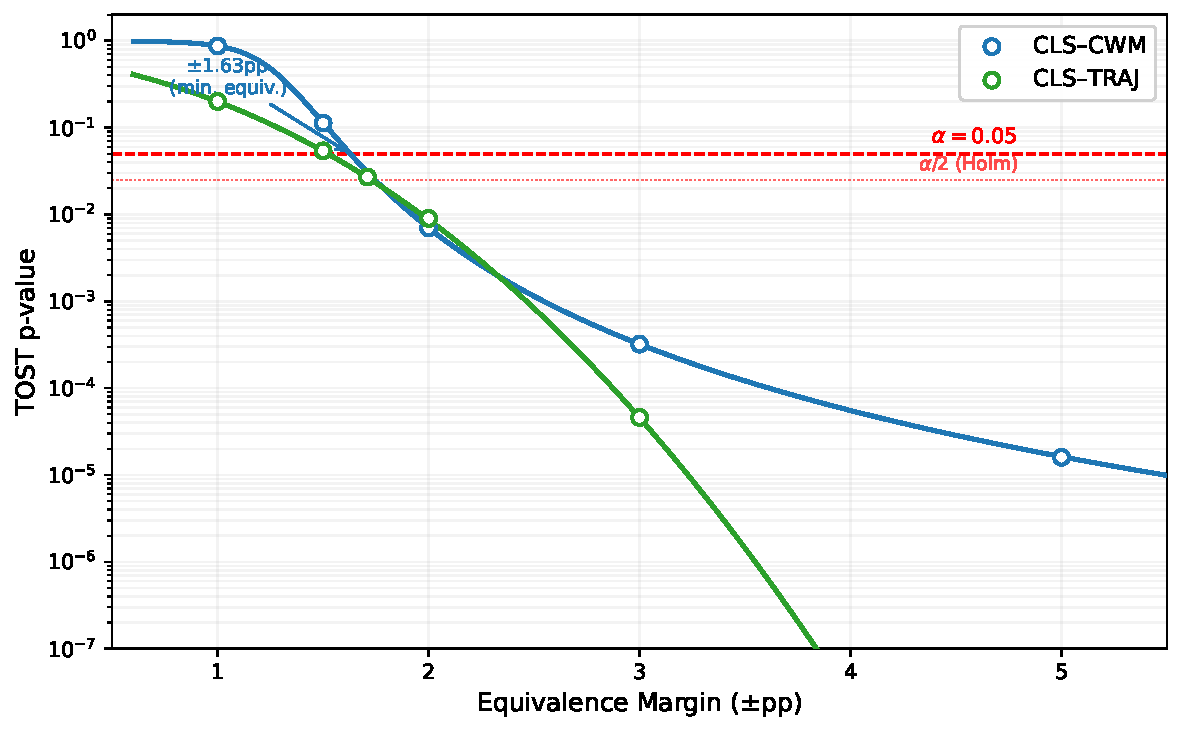
\includegraphics[width=0.78\columnwidth]{figures/paper/fig_tost_sensitivity.pdf}
\caption{TOST $p$-value as a function of equivalence margin. \cls{}--\cwm{} achieves equivalence at $\pm$1.63\pp{}; \cls{}--\traj{} crosses $\alpha{=}0.05$ near $\pm$1.8\pp{} but does not survive Holm correction. Log scale.}
\label{fig:tost_sensitivity}
\end{figure}

The minimum equivalence margin is $\pm$1.63\pp{}, 0.37\pp{} below our pre-specified $\pm$2\pp{} threshold. The $\pm$2\pp{} threshold was set based on deployment relevance rather than observed data: at function-level accuracy (85--88\%), a 2\pp{} per-test difference corresponds to ${\sim}$38 additional errors across 1,890 tests (${\sim}$2--3 problems out of 114), comparable in magnitude to between-seed standard deviation (0.37--0.97\pp{}) and checkpoint selection noise ($<$1\pp{}). Differences within this range do not reliably distinguish formulations from training noise in pipeline selection decisions. For \cls{}--\traj{}, the TOST at $\pm$2\pp{} yields $p{=}0.025$, nominally significant but not surviving Holm-Bonferroni correction at $k{=}5$ (adjusted $p{=}0.075$; Table~\ref{tab:holm}). The one-sided decomposition reveals the binding constraint: $p_{\text{upper}}{=}0.005$ ($\Delta < {+}2$\pp{} is well-confirmed) while $p_{\text{lower}}{=}0.025$ ($\Delta > {-}2$\pp{}) limits the overall TOST, consistent with \cls{} having mildly higher accuracy.

\paragraph{Robustness: seed-level vs.\ clustered bootstrap TOST.}
The primary TOST $p$-values use seed-level paired analysis (df${=}$4), treating each training seed as the unit of replication (\S\ref{sec:setup}). Under problem-level clustered bootstrap (resampling 114 problem clusters, 10K iterations), the \cls{}--\traj{} raw TOST $p$ decreases to ${\sim}$0.007 (Holm-adjusted $p{\approx}0.021$), which would confirm equivalence. We report the more conservative seed-level result ($p{=}0.025$, adjusted $p{=}0.075$) as primary, since training seeds are the true unit of replication; problem-level bootstrap pools within-seed observations and may understate between-seed uncertainty. For \cls{}--\cwm{}, both methods confirm equivalence ($p \leq 0.010$), so the choice does not affect conclusions.

\subsection{Bayesian ROPE Analysis}
\label{app:bayesian_rope}
To complement the frequentist TOST, we conduct a Bayesian equivalence analysis using a paired $t$-test with Jeffreys prior~\cite{kruschke2013bayesian,kruschke2018rejecting}. The marginal posterior for the mean accuracy difference follows a $t$-distribution with $n{-}1$ degrees of freedom. For \cls{}--\cwm{}, the posterior probability within the $\pm$2\pp{} ROPE is $P(\text{ROPE}) = 0.975$, and the 95\% highest density interval (HDI $= [{+}0.10, {+}2.00]$\,pp) falls entirely inside the ROPE, confirming equivalence under both continuous and HDI-based decision criteria. For \cls{}--\traj{} at per-test level, $P(\text{ROPE}) = 0.542$ (inconclusive; 95\% HDI $= [{+}0.35, {+}3.52]$\,pp extends beyond the ROPE), consistent with the TOST inconclusive result after Holm correction ($p_{\text{adj}} = 0.075$). At variant level, \cls{}--\traj{} equivalence is supported by the Bayesian criterion ($P(\text{ROPE}) = 0.970$, HDI $= [{-}2.00, {+}1.03]$\,pp), but the frequentist TOST remains inconclusive after Holm-Bonferroni correction ($p_{\text{adj}} = 0.075$; Table~\ref{tab:holm}). This discrepancy reflects differing treatments of multiplicity: Bayesian ROPE evaluates each comparison independently, while Holm correction penalizes across all $k{=}5$ primary tests. For \cls{}--\cwm{}, both frameworks agree (TOST $p_{\text{adj}}{=}0.028$, $P(\text{ROPE}){=}0.975$); for \cls{}--\traj{} per-test, both are inconclusive. We conservatively follow the Holm-corrected TOST in the main text and report \cls{}--\traj{} equivalence as inconclusive.

\paragraph{14B scaling evidence.} At 14B (3 seeds), the \cls{}--\cwm{} gap narrows to 0.43\pp{} and the \cls{}--\traj{} gap to 1.07\pp{}, both within the $\pm$2\pp{} margin. Seed-level TOST (df${=}$2) is inconclusive for equivalence in both pairs ($p{=}0.076$ for \cls{}--\cwm{}, $p{=}0.187$ for \cls{}--\traj{}), reflecting the severe power limitation of 3-seed comparisons (power ${\sim}$0.08 at $\pm$2\pp{} margin with df${=}$2). Bayesian ROPE provides moderate support: $P(\text{ROPE}){=}0.887$ for \cls{}--\cwm{} and $P(\text{ROPE}){=}0.780$ for \cls{}--\traj{}. Under problem-level clustered bootstrap, both comparisons reach significance ($p{=}0.0006$ and $p{=}0.043$ respectively), but this analysis treats within-seed observations as exchangeable, potentially understating between-seed uncertainty. The monotonic gap reduction (3.11\pp{} at 4B $\to$ 2.24\pp{} at 8B $\to$ 1.07\pp{} at 14B) favors a capacity-dependent convergence interpretation, though formal confirmation at seed level requires more training seeds.


\section{Variant-Level Effect Sizes}
\label{app:power}

Table~\ref{tab:variant_power} reports variant-level bootstrap confidence intervals for the repo-level formulation comparisons ($n{=}48$ variants). Following Hoenig and Heisey~\cite{hoenig2001}, we report minimum detectable effect (MDE) rather than post-hoc observed power.

\begin{table}[h]
\centering
\small
\caption{Variant-level bootstrap analysis ($n{=}48$). \cls{}--\cwm{} uses paired bootstrap (same variants, same seed); \cls{}--\traj{} uses unpaired bootstrap (per-variant \traj{} predictions not archived for pairing). MDE at $n{=}48$: ${\sim}$25\pp{}.}
\label{tab:variant_power}
\setlength{\tabcolsep}{6pt}
\begin{tabular}{llccc}
\toprule
\textbf{Comparison} & \textbf{Config} & \textbf{$\Delta$ (\pp{})} & \textbf{95\% CI} & \textbf{$p$} \\
\midrule
\multicolumn{5}{l}{\emph{\cls{} vs.\ \cwm{} (paired)}} \\
& Qwen3-8B & +29.17 & [10.42, 47.92] & 0.003 \\
& DeepSeek-6.7B & +35.42 & [18.75, 50.05] & ${<}$0.001 \\
\midrule
\multicolumn{5}{l}{\emph{\cls{} vs.\ \traj{} (unpaired)}} \\
& Qwen3-4B & $-$4.17 & wide & 0.740 \\
& Qwen3-8B & +8.33 & wide & 0.385 \\
& DeepSeek-6.7B & 0.00 & wide & 1.000 \\
\bottomrule
\end{tabular}
\end{table}

At $n{=}48$, the MDE is ${\sim}$25\pp{}. The \cls{}--\cwm{} gap (29--35\pp{}) exceeds this threshold, confirming that $n{=}48$ is sufficient to detect the observed divergence. The \cls{}--\traj{} gaps ($<$10\pp{}) fall well below the MDE: any true difference is too small to detect at this sample size, consistent with the function-level TOST equivalence (\S\ref{sec:equivalence}).

The \cls{}--\traj{} unpaired bootstrap produces wider confidence intervals than paired analysis would; \traj{} per-variant predictions were not archived in a format that permits pairing. The \cls{}--\cwm{} paired comparison uses \cls{} s123 vs.\ \cwm{} s42 (different seeds), but the CI lower bound of 10.42\pp{} far exceeds the seed noise observed in function-level experiments ($<$2\pp{}).


\section{Multiple Comparison Correction}
\label{app:holm}

Table~\ref{tab:holm} (main text) applies Holm-Bonferroni correction~\cite{holm1979} to the five primary statistical comparisons across this study ($k{=}5$, family-wise $\alpha{=}0.05$).

The two core claims survive correction: the repo-level \cls{}--\cwm{} divergence (adjusted $p{=}0.015$) and function-level \cls{}--\cwm{} equivalence (adjusted $p{=}0.028$). The function-level \cls{}--\traj{} equivalence does not survive correction (adjusted $p{=}0.075$). Under problem-level clustered bootstrap, the raw TOST $p$ decreases to ${\sim}$0.007 (adjusted $p{\approx}0.021$), which would confirm equivalence; we report the more conservative seed-level result ($p{=}0.025$) as primary, since training seeds are the true unit of replication.

\section{Mixed-Effects Regression}
\label{app:interaction}

We fit mixed-effects linear probability models (LPM) with heteroskedasticity-robust standard errors (HC1) to test the formulation$\times$complexity interaction formally~\cite{moulton1990}. We choose LPM because coefficients are directly interpretable as probability differences (percentage points), consistent with the reporting units in the main text; at these sample sizes ($n{\approx}56$K cross-complexity, repo-level pooled cross-model) and base rate range (0.6--0.9), LPM and logistic regression yield concordant conclusions for all primary effects~\cite{angrist2009mostly} (confirmed below).

\paragraph{Cross-complexity model (DeepSeek-Coder).} \texttt{correct $\sim$ formulation $\times$ complexity + (1|problem\_id)}, $n{=}56{,}480$ observations (\cls{} + \cwm{} $\times$ function + repo), 139 problem clusters. The \cwm{} main effect at function level is non-significant ($\hat{\beta}{=}-0.002$, $z{=}-0.25$, $p{=}0.805$); the \cwm{}$\times$repo interaction is highly significant ($\hat{\beta}{=}-0.219$, $z{=}-23.7$, $p{<}0.001$). \cwm{} and \cls{} are statistically indistinguishable at function level ($\Delta{=}-0.2$\pp{}, $p{=}0.805$) but diverge by 22\pp{} at repo level, confirming the complexity-dependent divergence is not an artifact of aggregation.

\paragraph{Repo-level cross-model model.} \texttt{correct $\sim$ formulation $\times$ model + (1|problem\_id)}, both model families, repo level only. \cwm{} deficit: $\hat{\beta}{=}-0.22$ ($-$22\pp{}, $z{=}-64.4$, $p{<}0.001$). Model effect: +1.1\pp{} for Qwen3 ($z{=}3.1$, $p{=}0.002$ in LPM; not significant under GEE, $p{=}0.449$). Formulation$\times$model interaction: +1.6\pp{} less \cwm{} degradation on Qwen3 ($z{=}2.8$, $p{=}0.006$ in LPM; not significant under GEE, $p{=}0.860$). Formulation dominates the predictable variance; model identity is directionally positive but specification-dependent. The 25-cluster random intercept structure limits effective degrees of freedom for the random effects; inferences on fixed effects (formulation, complexity) are robust as they pool across the full observation count.

\paragraph{Logistic regression robustness check.} To verify that LPM conclusions are not artifacts of the linear link function, we fit GEE logistic regression (binomial family, exchangeable working correlation, robust sandwich standard errors) to the same data. For the cross-complexity model, the \cwm{} main effect at function level has odds ratio (OR)$=$0.98 (95\% CI [0.86, 1.12], $p{=}0.771$) and the \cwm{}$\times$repo interaction has OR$=$0.31 ([0.15, 0.65], $p{=}0.002$). Average marginal effects are $-$0.2\pp{} (function) and $-$21.6\pp{} (repo), matching LPM coefficients within 0.3\pp{}. For the cross-model model, the \cwm{} deficit has OR$=$0.30 ([0.15, 0.63], $p{=}0.001$, AME$=$\,$-$21.1\pp{}). Direction, magnitude, and significance of all primary effects are concordant between LPM and logistic regression; minor discrepancies in secondary effects (model identity, formulation$\times$model interaction: $p{=}0.449$ and $p{=}0.860$ under GEE vs.\ $p{=}0.002$ and $p{=}0.006$ under LPM) reflect the GEE's more conservative cluster-robust inference with $k{=}25$ clusters. The discrepancy in secondary effects reflects cluster count: the cross-complexity model ($k{=}139$) yields reliable sandwich SEs, while the cross-model model ($k{=}25$) falls below the $k{\geq}40$ threshold recommended for stable cluster-robust inference~\cite{cameron2008bootstrap}.

\section{CWM Parseable Bias Analysis}
\label{app:parseable_bias}

Figure~\ref{fig:cwm_unparseable} (main text) summarises the unparseable rate contrast across complexity levels.

The default-to-pass assignment for unparseable \cwm{} outputs is not random with respect to instance difficulty. Unparseable instances have significantly higher pass rates than parseable ones (74.6\% vs.\ 68.3\%, $\chi^2$ $p = 5.9 \times 10^{-10}$), and \cls{} models achieve higher accuracy on unparseable instances (86.4\% vs.\ 79.1\%, $p = 3.3 \times 10^{-18}$). This indicates that \cwm{}'s parsing failures concentrate on simpler, pass-heavy instances where the majority-class default happens to be correct more often. Cross-model Jaccard overlap of unparseable instance sets is 0.46, confirming this pattern is instance-driven (specific inputs consistently cause parsing failure across models) rather than stochastic. The net effect is that \cwm{}'s reported accuracy is inflated by default-correct assignments on easy instances, while its effective discriminative accuracy on harder instances is substantially lower than the aggregate figure suggests.


\section{Threats to Validity (Full Analysis)}
\label{app:threats}

We identify five potential confounds and assess their impact on our conclusions.

\paragraph{Checkpoint selection.} Val-based selection is unavailable for runs with NaN validation loss (DeepSeek \cwm{} repo-level runs, DeepSeek \cls{} s123), which default to the final epoch checkpoint. A checkpoint ablation on Qwen3-8B \cls{} s42 quantifies this confound: epoch~1 (ckpt-2200) achieves 85.34\%, val-selected (ckpt-3600) 84.48\%, and final epoch (ckpt-6633) 85.29\%, a $<$1\pp{} range. The val-selected checkpoint is the lowest, indicating no upward bias from checkpoint selection. The Qwen3-8B \traj{} comparison (epoch 2: 72.92\% vs.\ epoch 3: 70.83\%) shows a slightly larger ${\sim}$2\pp{} shift. For \cwm{}, the convergence analysis (Appendix~\ref{app:cwm_convergence}) shows eval loss at the final epoch is 1.8$\times$ its minimum; however, early-stopped checkpoints retain high unparseable rates, leaving the qualitative ranking unchanged.

\paragraph{\cwm{} convergence analysis.}
\label{app:cwm_convergence}
Qwen3-8B \cwm{} repo-level eval loss reaches its minimum within ${\sim}$5\% of training (step 300--400 of 6{,}633) and increases monotonically thereafter, with no plateau or recovery (Table~\ref{tab:cwm_convergence}). This pattern is consistent across all three seeds, confirming systematic overfitting to trace generation rather than stochastic variation. The final-epoch eval loss is ${\sim}$1.8$\times$ the optimal value. By contrast, function-level \cwm{} achieves \cls{}-equivalent accuracy (TOST $p{=}0.007$) with the same training recipe, indicating that the overfit is specific to repo-level output complexity. Cross-model validation: a DeepSeek-Coder early-stopped checkpoint (s123, epoch~1) achieves 75.45\% versus 57.31\% at epoch~3 (s123; +18.14\pp{}), but retains 66.4\% unparseable rate, confirming that format collapse emerges early and is not a late-training artifact. No epoch-level checkpoint is available for Qwen3 CWM (only step-level checkpoints at steps 300/400 and late steps ${\geq}$5800; continuous epoch checkpointing was not enabled for this training run). The convergence analysis (Table~\ref{tab:cwm_convergence}) shows eval loss minimum at step 300--400 across all three Qwen3 seeds, consistent with DeepSeek-Coder's epoch-1 improvement, providing cross-model evidence that the overtraining pattern generalizes. An early checkpoint (step 400, ${\sim}$6.5\% of training, s42) yields 65.17\% repo-level accuracy with 63.7\% unparseable rate, comparable to or below final-epoch performance (66.93--67.33\% accuracy, 60.4--63.9\% unparseable; s123/s456 at step 6633). This rules out late-training format degradation: collapse is present from early training, and the optimal eval-loss checkpoint does not recover repo-level accuracy. A later checkpoint (step 6100, s42, seq8192) achieves 69.50\% test accuracy despite substantially higher validation loss than val-best ckpt-400 (64.36\%), suggesting that validation loss may not be a reliable proxy for test-set performance in \cwm{} repo-level evaluation.

\begin{table}[h]
\centering
\small
\caption{\cwm{} repo-level eval loss across training (Qwen3-8B, 3 seeds). Minimum is reached at step 300--400 (${\sim}$5\% of training); subsequent training monotonically increases loss.}
\label{tab:cwm_convergence}
\begin{tabular}{lccc}
\toprule
Step & s42 & s123 & s456 \\
\midrule
300 & 0.291 & \textbf{0.288} & \textbf{0.277} \\
400 & \textbf{0.286} & 0.306 & 0.283 \\
1000 & 0.333 & 0.336 & 0.351 \\
3000 & 0.445 & 0.453 & 0.435 \\
6600 & 0.521 & 0.517 & 0.507 \\
\bottomrule
\end{tabular}
\end{table}

\paragraph{Evaluation sequence length.} \cwm{} accuracy varies by ${\sim}$9\pp{} across evaluation sequence lengths for the same checkpoint (seq2048: ${\sim}$65\% vs.\ seq4096: ${\sim}$56\%), driven by unparseable-rate differences that propagate through majority-class default assignment. \cls{} is invariant to this parameter. Cross-model \cwm{} comparisons use different eval lengths (Qwen3: 8192, DeepSeek: 4096) and are not directly comparable in absolute terms. A matched-sequence evaluation shows ${\sim}$1.5\pp{} difference for \cls{} (Appendix~\ref{app:ablations}), insufficient to explain the 18--26\pp{} gap. Furthermore, increasing Qwen3-8B \cwm{} evaluation from seq4096 to seq8192 \emph{raises} the unparseable rate (63.7\%$\to$73.8\%) while changing accuracy by only 0.81\pp{} (64.36\%$\to$65.17\%); giving the model more generation budget worsens format compliance rather than improving it, confirming that format collapse is a structural bottleneck rather than a truncation artifact. Practitioners must standardize evaluation sequence length for generation-based formulations.

\paragraph{Preprocessing.} DeepSeek \cls{} accuracy ranges from 82.61\% (s42, drop preprocessing) to 74.93\% (s123, truncate preprocessing), a 7.68\pp{} spread that conflates preprocessing strategy, checkpoint selection method, and seed. The two strategies produce different effective training sets (67,343 vs.\ 70,748 samples) and different checkpoint selection regimes. The qualitative ranking \cls{} $>$ \cwm{} holds under both strategies (Table~\ref{tab:taxonomy}).

\paragraph{\traj{} training regime.} \traj{} uses a different training configuration: smaller training set (${\sim}$400 repo-level variants vs.\ ${\sim}$70K per-test instances), higher learning rate ($2{\times}10^{-4}$ vs.\ $5{\times}10^{-5}$), and variant-level labels. This asymmetry is inherent to the formulation (trajectory-level labels are only available at variant granularity), but precludes training-data-controlled comparison at repo level. The downsample ablation confirms the \cls{} formulation advantage persists at matched data volume (80.74\% vs.\ 72.92\%; Appendix~\ref{app:downsample}), though it controls for training volume but not label granularity (per-test vs.\ variant-level). Crucially, \traj{} achieves statistical equivalence with \cls{} at function level (${\leq}$1.3\pp{}, \S\ref{sec:func_results}), demonstrating the formulation itself is viable; the repo-level gap attribution remains uncertain: data volume (${\sim}$400 variants vs.\ ${\sim}$70K per-test instances) and label granularity (variant-level vs.\ per-test) are both plausible confounds that cannot be separately controlled.

\paragraph{\cwm{} scale and pretraining.} Our \cwm{} baseline uses 4--8B LoRA fine-tuning without execution trace pretraining. The original Code World Model~\cite{meta2025cwm} uses 32B parameters with mid-training on execution traces, a fundamentally different training regime. At larger scale or with execution-trace pretraining, the generation bottleneck observed here may diminish: larger models produce more coherent long-form outputs, and execution trace exposure may improve output format compliance. This is the primary limitation: all repo-level \cwm{} conclusions are conditional on the ${\leq}$8B LoRA regime.

Despite these confounds, the repo-level \cls{}--\cwm{} gap (18--26\pp{}) exceeds any single assessed confound. Even under worst-case compounding (${\sim}$11.5\pp{}), the gap retains ${\geq}$7.5\pp{} margin; confounds predominantly disadvantage \cwm{}. However, correlated confounds and limited seed coverage mean definitive causal attribution requires multi-seed replication. At $n{=}48$, the minimum detectable effect (MDE) is ${\sim}$25\pp{}~\cite{hoenig2001}; the \cls{}--\cwm{} gap (29--35\pp{}) exceeds this threshold, while the \cls{}--\traj{} gap ($<$10\pp{}) falls below it, consistent with our TOST equivalence finding. Holm-Bonferroni correction across the five primary comparisons ($k{=}5$; Table~\ref{tab:holm}) confirms the \cls{}--\cwm{} gap (adjusted $p{=}0.015$) and function-level \cls{}--\cwm{} equivalence (adjusted $p{=}0.028$); function-level \cls{}--\traj{} equivalence does not survive correction (adjusted $p{=}0.075$), nor does the repo-level \cwm{}--\traj{} comparison (adjusted $p{=}0.078$). The consistent direction across both model families and all tested configurations supports a formulation-level explanation, though definitive causal attribution requires future experiments addressing each confound individually.


\paragraph{Extended validity discussion.}
\label{app:limitations}
The same-size 4B comparison uses a single seed; \cls{} 4B seed 123 (val-best ckpt-800) achieves only 75.33\% test accuracy (+2.4\pp{} above majority baseline); val-best selection at an early checkpoint (step 800) amplifies the val-test distribution shift observed across all configurations. The \cwm{} 8B comparison uses 3 seeds per model. The validation and test sets have zero problem overlap but differ in mutation type composition (Table~\ref{tab:mutation_distribution}): \texttt{operator\_swap} shifts from 19.1\% (val) to 34.3\% (test), the largest single-type distribution mismatch (+15.2\pp{}). All repo-level results use val-selected checkpoints, and checkpoint selection variance could contribute to observed differences. Our training data is synthetically constructed from mutation operators rather than real developer patches. While mutation testing literature establishes that mutants are reasonable proxies for real faults in test effectiveness studies~\cite{andrews2005mutation,just2014mutants}, these findings concern mutation \emph{adequacy} (whether tests that kill mutants also detect real faults), not whether verifiers trained on mutants transfer to real patches. However, the coupling effect underlying these results supports \emph{relative ranking} validity: a domain shift from synthetic mutations to real bugs may affect absolute accuracy levels, but our core finding (that formulation choice matters at repo level but not function level) concerns relative performance ordering, which is expected to be preserved under distributional shifts that affect all formulations equally. The synthetic-to-real transfer gap for absolute accuracy remains untested. The \traj{} training configuration differs from \cls{}/\cwm{}: smaller training set (${\sim}$400 vs.\ ${\sim}$70K instances), different learning rate ($2{\times}10^{-4}$ vs.\ $5{\times}10^{-5}$), and variant-level evaluation ($n{=}48$ vs.\ per-test $n{=}9{,}784$). The function-level \cls{}--\traj{} TOST equivalence ($p = 0.025$, seed-level paired, $\pm$2\pp{}) is computed on 523 matched variant-level instances across 5 seeds; 2 of 5 seeds use NF4 quantization. Restricting to three bfloat16 seeds yields a comparable mean gap ($-$0.45\pp{}) but wider confidence interval (df${=}$2); the TOST $p$-value increases to 0.128, which reflects reduced statistical power rather than a shift in the point estimate. The NF4 seeds contribute precision (narrowing the CI) without shifting the mean, consistent with precision being comparable across both quantization levels at function level. Repo-level \cls{}--\traj{} comparison should be interpreted with caution due to configuration and granularity differences.

\paragraph{Domain contrast with generative verification in math reasoning.}
GenRM~\cite{hosseini2025genrm} demonstrates that generative verifiers outperform discriminative ones for math reasoning. Our results reveal a domain-specific divergence: in code repair verification, the generative formulation (\cwm{}) does not outperform the discriminative one (\cls{}), and degrades sharply at repository level. The key difference is output space structure: math reasoning generates natural-language solution traces with flexible formatting, whereas code execution output requires exact syntactic compliance (specific variable values, error messages, stack traces). This structural constraint makes format collapse, absent in math verification, the dominant failure mode for code \cwm{} at repo level (53--74\% unparseable). The domain contrast suggests that the generative verification advantage is contingent on output space complexity rather than being a universal property of verifier architecture.

\section{Use of AI Assistance}
\label{app:ai-assistants}
We used Claude for coding, code drafting, debugging, and language polishing.


\end{document}
